\documentclass[pra,superscriptaddress,reprint,amsmath,amssymb,nofootinbib]{revtex4-2}

\usepackage{graphicx}
\usepackage{dcolumn}
\usepackage{subfiles} 
\usepackage{bm}
%for nice coloured hyperlinks:
\usepackage[usenames,dvipsnames]{xcolor}
\usepackage[pdftex,plainpages=false,colorlinks=true]{hyperref}
\usepackage[toc,page,title,titletoc,header]{appendix} 
\usepackage{multirow}
\usepackage{tabularx}
%\usepackage[bottom]{footmisc}
%\usepackage{caption}
%\usepackage{subcaption}
%\usepackage[bottom]{footmisc}
%\usepackage{soul}
\usepackage{algorithm}
\usepackage{algpseudocode}
\algnewcommand{\To}{\textbf{To }}
\algnewcommand\Input{\item[\textbf{Initialisation:}]}%
\algnewcommand\Output{\item[\textbf{Output:}]}%
\usepackage{booktabs}

%%%%%%%%%%%%%%%%%%%%%%%%%%%%%%%%%%%%%%%%%%%%%%%%%%

%%%%% AUTHORS - PLACE YOUR OWN COMMANDS HERE %%%%%

% notes
\newcommand{\han}{\textcolor{orange}}
\usepackage[caption=false]{subfig}

%\usepackage[section]{placeins} %ensures figures go in their section e.g https://tex.stackexchange.com/questions/279/how-do-i-ensure-that-figures-appear-in-the-section-theyre-associated-with


% units
\newcommand{\Hz}{\mathrm{Hz}}
\newcommand{\ms}{\mathrm{ms}}
\newcommand{\secs}{\mathrm{s}}


% variables
\newcommand{\omegahigh}{\omega_{\mathrm{high}}}
\newcommand{\omegalow}{\omega_{\mathrm{low}}}
\newcommand{\fgw}{f_{\mathrm{gw}}}
\newcommand{\fline}{f_{\mathrm{line}}}

\newcommand{\CSOneName}{\texttt{H1:PEM-CS\_MAINSMON\_EBAY\_1\_DQ}}

\newcommand{\StrainChanName}{\texttt{L1:DCS-CALIB\_STRAIN\_C01\_AR}}
\newcommand{\PEMChanName}{\texttt{L1:PEM-CS\_MAINSMON\_EBAY\_1\_DQ}}
%%%%%%%%%%%%%%%%%%%%%%%%%%%%%%%%%%%%%%%%%%%%%%%%%%




%\let\oldfootnote\footnote
%\renewcommand{\footnote}[1]{%
%	\begingroup%
%	\linespread{1}%    % <- linespread for footnote: 1, 1.1, 1.2 etc
%	\oldfootnote{#1}%
%	\endgroup%
%}
%
%\interfootnotelinepenalty=10000






%%%%%%%%%%%%%%%%%%% TITLE PAGE %%%%%%%%%%%%%%%%%%%

\begin{document}
\preprint{}

\title[test short title]{Adaptive cancellation of power grid interference in continuous gravitational wave searches with a hidden markov model}% Force line breaks with \\
%\thanks{this would be a footnoted on the first page}%

%\input{authors.tex}

\author{Author 1, Author 2, etc. Kimpson, Suvrova, Liu, Melatos, Middleton, Evans, Moran, Meyers, any others?}
\date{\today}% It is always \today, today,
             %  but any date may be explicitly specified


\begin{abstract}
		Continuous gravitational wave (GW) searches are commonly hampered by long-lived, narrow peaks in the instrumental frequency spectra known as `lines'. Candidate GW signals which lie within frequency bands with known lines are typically vetoed. In this work we demonstrate a new line subtraction method based on adaptive noise cancellation (ANC). ANC is common in electrical engineering applications, including for processing audio and biomedical signals. We show how ANC can be used in conjunction with a Viterbi search to track spin-wandering continuous wave signals near the LIGO 60 Hz line. 
\begin{description}
\item[DOI]
\end{description}
\end{abstract}



\maketitle	


\section{Introduction} \label{sec:intro}
Instrumental noise artifacts in gravitational wave (GW) searches with terrestrial, long-baseline interferometers are classified according to their duration and spectral properties.  Short-lived, non-stationary recurrent noise events such as optomechanical glitches typically last for seconds and exhibit distinctive spectral signatures, e.g they can be chirp-like \cite{Blackburn2008,Aasi2012,Aasi2015,DetCharGW150914:2016,Glanzer2023}. Long-lived, quasi-stationary, broadband noise sources include seismic disturbances at low frequencies, test mass thermal fluctuations at intermediate frequencies, and photon shot noise at high frequencies \cite{AasiEtAlAdLIGO:2015,LIGOnoiseguide,VIROGnoise,Akutsu2021PTEP,Nguyen2021}. Long-lived narrowband spectral artifacts - termed instrumental lines - are caused by electrical subsystems (e.g. mains power, clocks, oscillators), mechanical subsystems (e.g. test mass and beam-splitter violin modes) and calibration processes \cite{CovasEtAl:2018}, although often the origin of a specific feature is unknown. Instrumental lines are disruptive, especially for continuous wave (CW) searches where the target astrophysical signal is quasi-monochromatic and resembles the noise artifact spectrally. Many above-threshold candidates discovered in CW searches to date are vetoed because they coincide with known instrumental lines \cite{Piccinni2022,Riles2023,Wette2023}, for instance, in CW searches involving data from Observing Run 3 (O3) with the Laser Interferometer Gravitational Wave Observatory (LIGO), Virgo and the Kamioka Gravitational Wave Detector (KAGRA)  \cite[e.g.][]{Ligo_lineveto1,ligo_lineveto2,ligo_lineveto3} \newline 


Several techniques have been implemented by the LIGO-Virgo-KAGRA (LVK) collaboration to identify, characterize and suppress instrumental noise artifacts \cite{Davis2021,Davisgalaxies10010012}. Some techniques identify and veto an artifact (or gate a segments of the data) based on its time-frequency signature \cite{Abbott2018CQVeto,Lee2021,Steltner2022Ph}. Other techniques perform offline noise subtraction with reference to auxiliary data from physical environmental monitors (PEMs) \cite{Driggers2012RScI,Tiwari2015,Davis2019,Driggers2019}. PEMs can be used to witness correlated noise and generate a reference signal directly or elucidate and quantify multichannel couplings \cite{Jung2022PRD,marin1997}. Finally some techniques are based on machine learning \cite{Cuoco2020,Vajente2020PhR,OrmistonEtAl:2020,Yamamoto2023}. In CW searches specifically, the distinctive amplitude and frequency (Doppler) modulations associated with the Earths rotation and revolution can be exploited to discriminate between terrestrial noise artifacts and astrophysical signals \cite{Zhu2017PhRvD,JonesPhysRevD.106.123011}.  \newline 

In most  of the situations above, the practical effect of an instrumental line is to excise the relevant part of the observing band from a CW search. That is, if an above threshold CW search candidate coincides with a known instrumental line, the candidate is vetoed under current practice without further analysis, such as comparing the expected strength of the noise line with the measured strength of the candidate \footnote{A regularly updated log of narrowband instrumental lines in the LVK detector is maintained at \href{https://dcc.ligo.org/LIGO-T2100200/public}{dcc.ligo.org/LIGO-T2100200/public} for public reference}. In this paper we take a first step towards lifting the above limitation. We introduce an adaptive noise cancellation (ANC) scheme  based on an adaptive recursive least squares (ARLS) method which suppresses narrowband noise proportional to a known PEM reference signal. We then apply the ANC scheme to a CW search algorithm based on a hidden Markov model (HMM) which detects and tracks quasi-monochromatic GW signals with wandering frequency and has been tested and validated thoroughly in multiple LVK searches \cite{Suvorova2016PhRv,Piccinni2022,Riles2023,Wette2023}. We demonstrate with synthetic data that the ANC scheme and HMM algorithm together can successfully detect a GW signal lying under the 60Hz mains power line, if the signal exceeds a well-defined minimum amplitude. The approach extends naturally to other instrumental lines, a topic for future work. \newline 

The paper is organized as follows. In Section \ref{sec:pgi} we outline our mathematical model for the 60Hz mains power spectral line and the PEM reference signal, and justify the assumptions of the model by reference to the strain and environmental data from the LIGO Livingston interferometer.  In Section \ref{sec:method} we introduce ANC formulated as an ARLS method. We go on in Section \ref{sec:results} to deploy the ANC method in conjunction with an HMM Viterbi solver applied to synthetic GW strain data and demonstrate the successful recovery of a monochromatic GW signal.  


\section{Power grid interference} \label{sec:pgi}
The goal of this paper is to detect a quasi-normal GW signal in a data stream contaminated by two kinds of noise: additive Gaussian noise which is fundamental and irreducible, and additive non-Gaussian interference from a long-lived narrow spectral feature which can be filtered out in principle given an accurately measured reference signal. For this work we consider the spectral line at 60 Hz that results from the North American alternating current power grid as the additive non-Gaussian interference. In Section \ref{sec22} we briefly review the 60 Hz LIGO interference line before proceeding in Section \ref{sec21} to specify the assumed mathematical forms of the interference and reference signals. In Section \ref{sec23} we justify the assumptions of Section \ref{sec21} by analysing differential arm length (DARM channel) and environmental (power grid monitoring) data from the LIGO interferometers. 


\subsection{LIGO 60 Hz Interference}  \label{sec22}
%Useful literature: https://journals.aps.org/prd/pdf/10.1103/PhysRevD.97.082002

LIGO data contains multiple long-duration narrow lines (e.g. Fig. \ref{fig:strainSensitivity}) in addition to the usual Gaussian noise. The provision of mains power electricity in North America via an alternating current with frequency 60 Hz leads to a line in the LIGO data at the corresponding frequency. The coupling between the mains power and the gravitational wave data channel can occur since the performance of the high-sensitivity electronic components within LIGO varies with respect to the input power voltage. Additionally, the magnetic fields that arise from the AC mains supply can couple with the magnets on the LIGO optical components. Whilst some spectral lines are static, the 60Hz line wanders in time, due to variations in the load in the North America power grid at any one time (e.g. Fig. \ref{fig:powerCascade}). This time variation can further impact the detector sensitivity over a broader frequency band. For a full review of LIGO spectral artifacts, including the 60 Hz line, we refer the reader to \cite{CovasEtAl:2018}.
\begin{figure}
	\begin{center}
		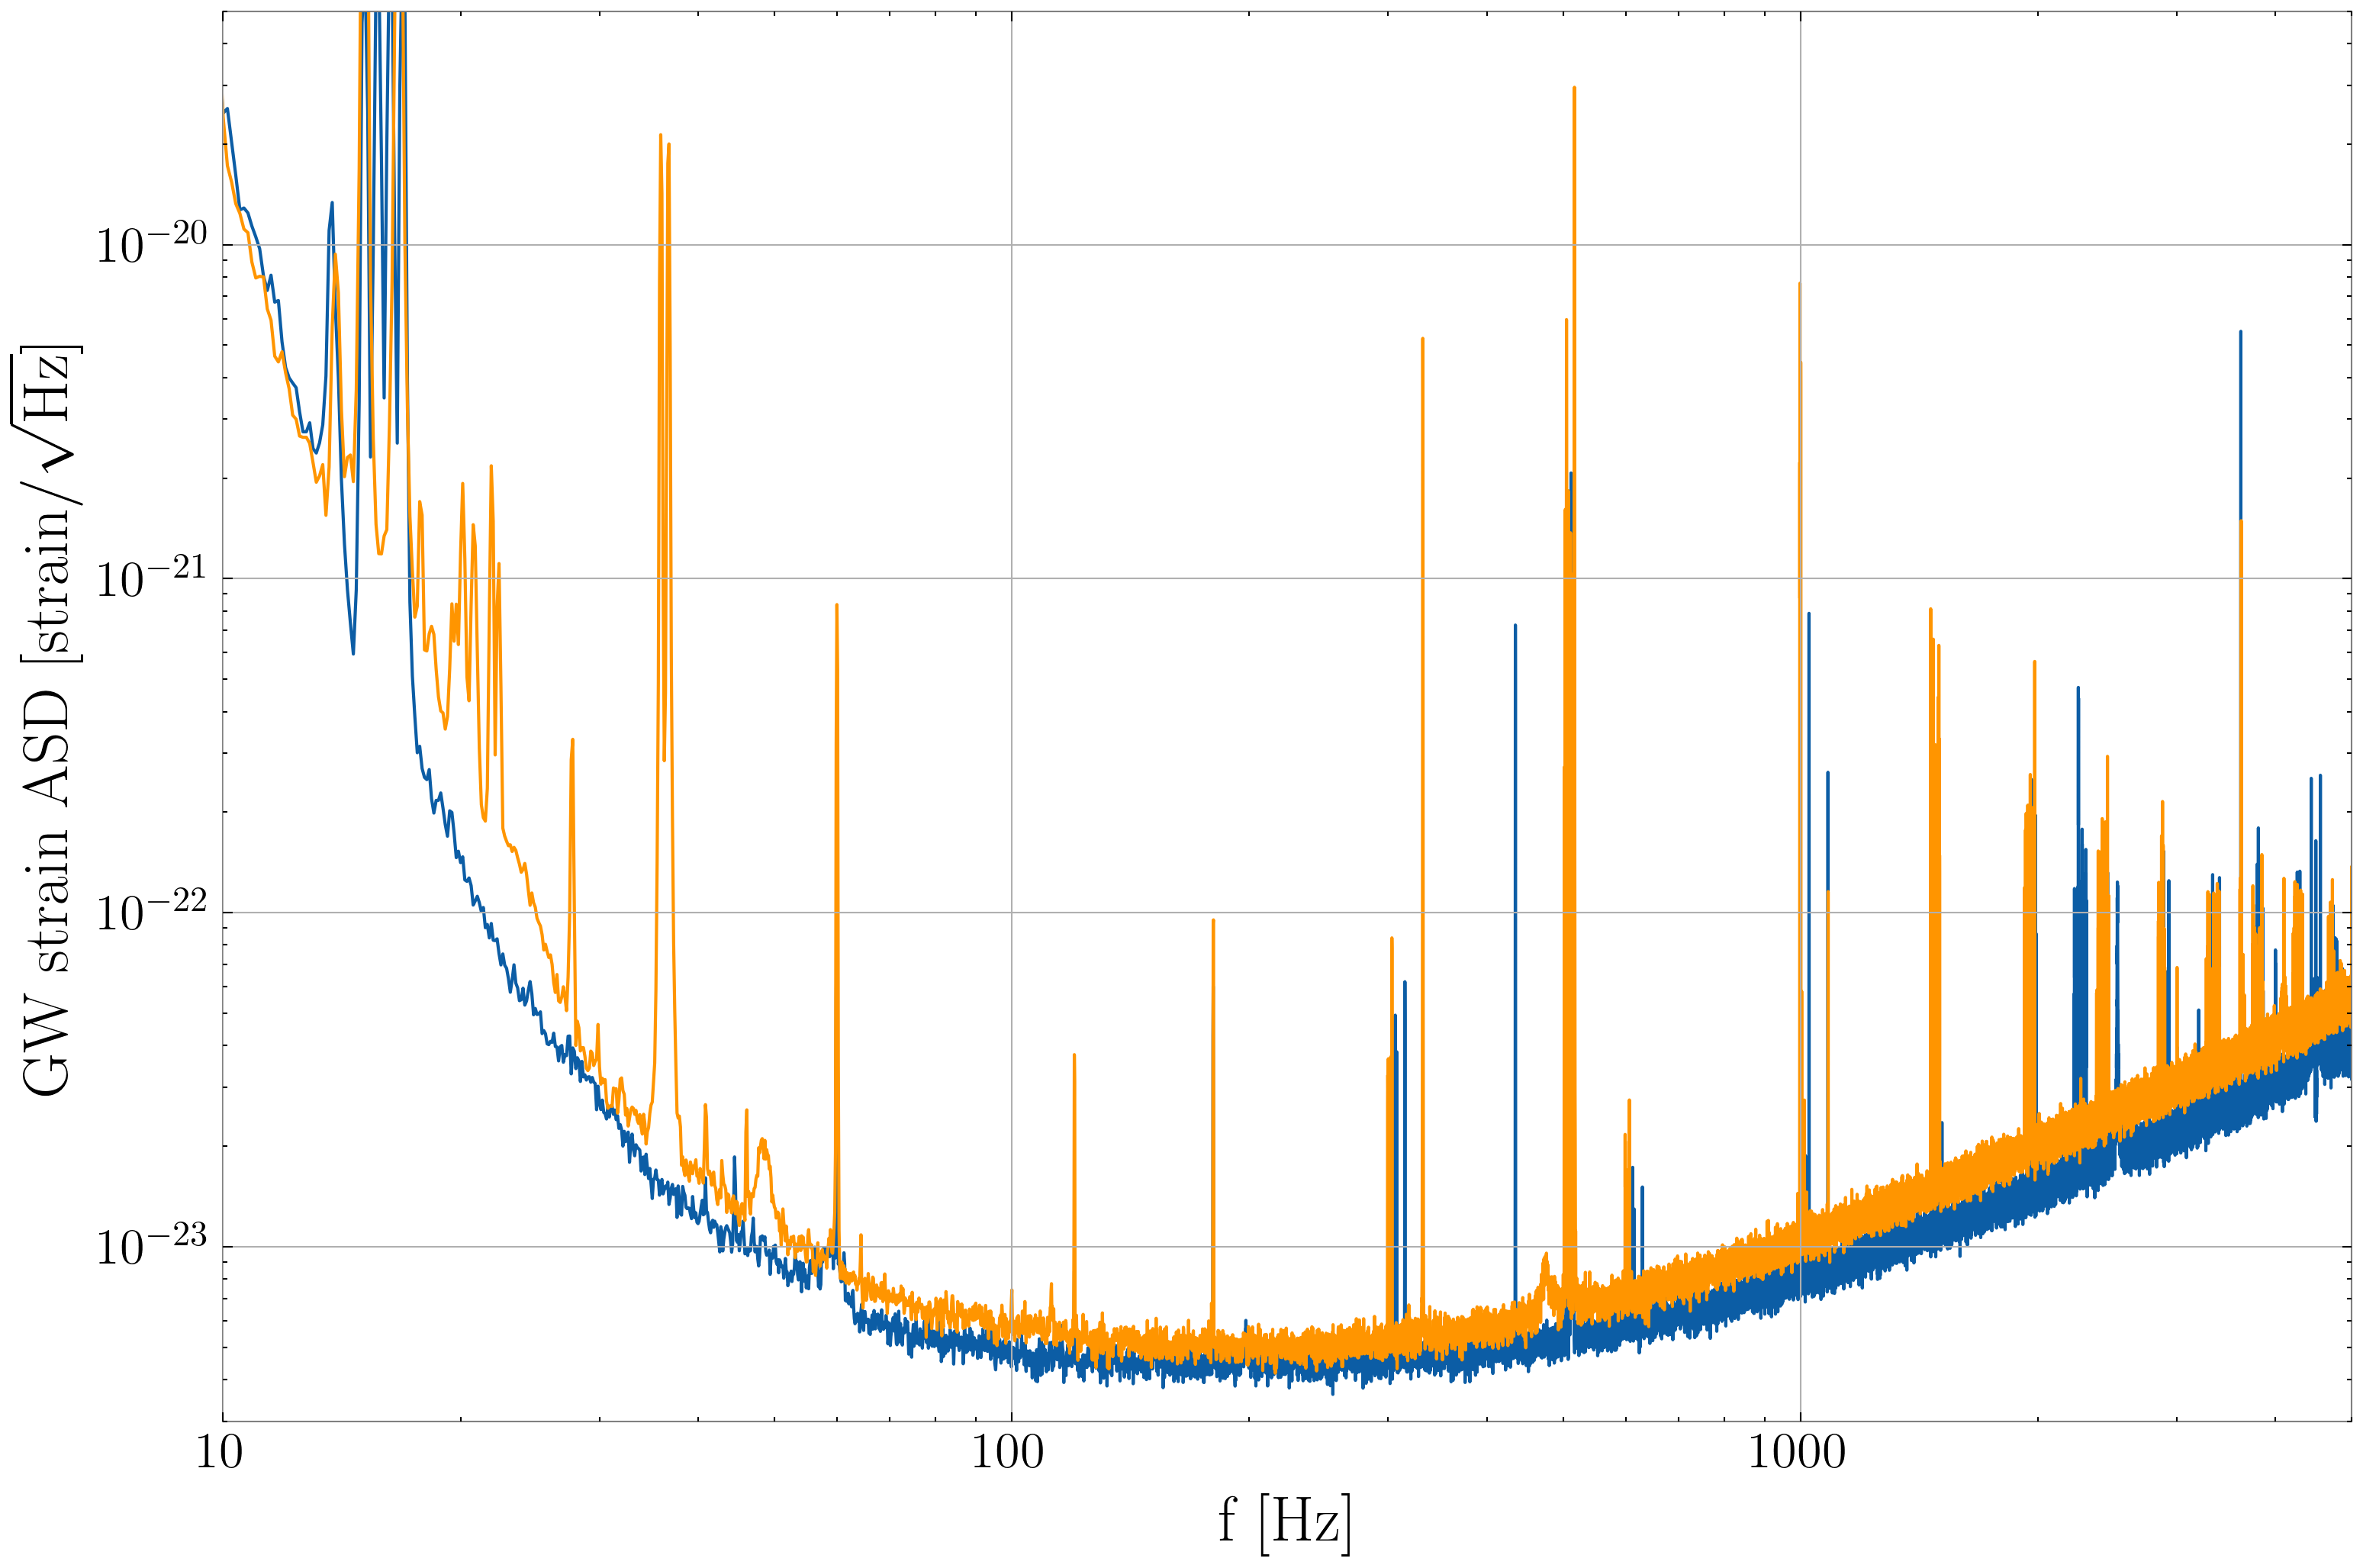
\includegraphics[width=\columnwidth]{images/sensitivity}
	\end{center}
	\caption{Sensitivity plot for LIGO-Hanford (orange) and LIGO-Livingston (blue) for a snapshot of data ($\sim 10$ minutes) from O3 (channel \texttt{*:DCS-CALIB\_STRAIN\_C01\_AR}, see Ref.~\cite{LIGO_O3, GWOSC:online}. The spectral line at $60\,{\rm Hz}$ is clearly visible, along with multiple other instrumental lines at other frequencies.}\label{fig:strainSensitivity}
\end{figure}
\begin{figure}
	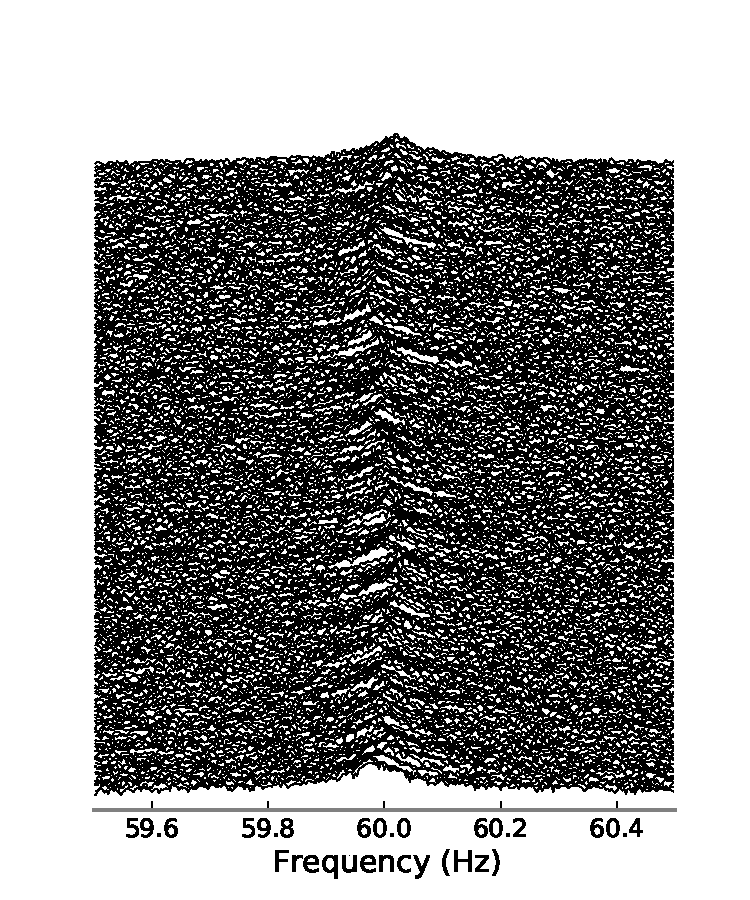
\includegraphics[width=\columnwidth]{images/powerCascade}
	\caption{Cascade plot showing the amplitude spectral density of the Hanford PEM monitor \CSOneName~ (corner station, phase 1) over time. Each trace corresponds to $320\,{\rm s}$ ($\approx 5\,{\rm min}$) of data ($210$ lines plotted). The wandering of the 60Hz instrumental line about its central value can be seen.
	}\label{fig:powerCascade}
\end{figure}
% the script for this plot is here on CIT
%/home/hannah.middleton/repositories/powerlines/powergridlines/plots/asd




%At each detector there are nine PEM for the power grid monitoring all three phases of power at the corner and two end stations at a sample rate of $1024\,{\rm Hz}$. 
%https://arxiv.org/abs/1903.03866 useful for Jaranowski discussion
\subsection{Statement of the problem: signal and noise models}  \label{sec21}
Let $x(t)$ denote the scalar time series output by the ``science" or strain channel of a LIGO-like long baseline interferometer. Suppose that $x(t)$ is sampled at discrete times $t_n$, with $1 \leq n \leq N$ and uniform sampling interval $\Delta t = t_n - t_{n-1}$. Let $r(t)$ denote the scalar time series output by the environmental channel relevant for filtering interference; here $r(t)$ is of one of the three phases of mains power measured at some reference point in the detector. The reference signal is usually sampled less frequently than $x(t)$ at discrete times $t_{n_k}$, with $1 \leq k \leq K$ and $1 \leq n_k \leq N$. We assume for the sake of convenience that every $t_{n_k}$ coincides with some $t_n$ for all $k$, but the condition is not essential. \newline 

The strain channel is composed of a gravitational wave signal $h(t)$, non Gaussian interference $c(t)$ (sometimes called ``clutter") and Gaussian noise $n(t)$ in a linear combination:
\begin{eqnarray}
	x(t) = h(t) + c(t) + n(t) \ .
	\label{eq:data}
\end{eqnarray}
 In this paper the gravitational wave signal takes the form predicted by \citet{Jaranowski1998} for a biaxial rotor, e.g. a neutron star (NS) emitting continuous gravitational waves at multiples of the star spin frequency $f_{\star}$. The GW signal is quasimonchromatic, amplitude-modulated by the rotation of the Earth and frequency modulated by the Earth's orbital motion. The noise $n(t)$ is white with $\langle n(t_n) n(t_{n'})\rangle = \sigma_n^2 \delta_{n n'}$. Noise samples $n(t_n)$ are drawn from a Gaussian distribution with zero mean and variance $\sigma_n^2$. The interference clutter $c(t)$ takes a form determined by instrumental processes but is generally a long-lived narrow spectral feature. We can relate $c(t)$ to the instrumental voltage $r(t)$ in the following. \newline 
 
 
 Mains power is characterized by three properties. First, the frequency is maintained at a constant value across the grid to to a good approximation by internal grid mechanisms (effectively a phase locked loop), with central frequency $f_{\rm ac} = 60$ Hz in North America. A slow periodic modulation occurs around $f_{\rm ac}$ with a small amplitude $\Delta f_{\rm ac} \lesssim 0.5$ Hz and period $P$ which wanders randomly and uniformly in the range $0 \leq P \leq P_{\rm max}$. Secondly, the phase $\Theta(t)$ of the voltage $r(t)$ wanders stochastically. We assume that the phase noise is white and Gaussian, with $n_{\Theta}(t_n)$ drawn from a Gaussian distribution with zero mean and variance $\sigma_{\Theta}^2$, and $\langle n_{\Theta} (t_n) n_{\Theta} (t_{n'})\rangle = \sigma^2_{\Theta} \delta_{n n'}$. Third, the voltage amplitude, $A_r(t)$, is random. We assume that samples $A_r(t)$ are distributed uniformly within $[A_{\rm ac} - \Delta A_{\rm ac} , A_{\rm ac} + \Delta A_{\rm ac}]$. We can then write the reference voltage as,
 \begin{eqnarray}
 	r(t) = A_r(t_n) \cos \left[ 2 \pi f_{\rm ac} t + \Theta(t)\right] +n_r(t_n) \ ,
 	\label{eq:voltage}
 \end{eqnarray}
with
 \begin{eqnarray}
\Theta(t) = 2 \pi \Delta f_{\rm ac} \cos\left(\frac{2 \pi t}{P(t_n)}\right) + n_{\Theta} (t_n) \ ,
\label{eq:voltage_theta}
\end{eqnarray}
%\begin{align}
%	r(t) &= \nonumber \\
%	& A_r(t_n) \cos \left( 2 \pi f_{\rm ac} t + 2 \pi \Delta f_{\rm ac} \cos\left(\frac{2 \pi t}{P(t_n)}\right) + n_{\Theta} (t_n)\right) \nonumber \\
%	& +w(t_n)
%	\label{eq:voltage}
%\end{align}
for $t_n \leq t \leq t_{n+1}$. That is, at time $t_n$, random variables $A_t(t_n)$, $P(t_n)$ and $n_{\Theta} (t_n)$ are drawn from the distribution $\mathcal{U}[A_{\rm ac} - \Delta A_{\rm ac},A_{\rm ac} + \Delta A_{\rm ac} ]$, $\mathcal{U}[0, P_{\rm max}]$, and $\mathcal{N} [0, \sigma_{\Theta}^2]$ respectively. Equation \eqref{eq:voltage} then runs forward over an interval of length $\Delta t$. Hence $r(t)$ is discontinuous at each sampling time. In Equation \eqref{eq:voltage}, $n_r(t_n)$ is the reference signal measurement noise at $t_n$, assumed to be white and Gaussian with $r_r(t_n)$ drawn from a Gaussian with zero mean and variance $\sigma_r^2$. All the white measurement and process noises are assumed independent. \newline 

Mains power couples into the strain channel in various complicated ways, e.g. through electronic devices, or inductively through ambient magnetic fields. A central assumption in this work is that the interference in the strain channel is an exact, amplitude-scaled replica of the reference signal up to a delay $\tau_{\rm delay}$ which is attributed to spatial propagation effects between the reference measurement front and the interferometer mirrors or dark front. Hence we can express the interference clutter as, 
 \begin{eqnarray}
	c(t) = A_c(t'_n) \cos \left[ 2 \pi f_{\rm ac} t' + \Theta(t')\right] \ ,
	\label{eq:vclutter}
\end{eqnarray}
for $t_n \leq t \leq t_{n+1}$ and $t' = t_n - \tau_{\rm delay}$. The amplitude $A_c$ is distributed as $\mathcal{U}[A_{\rm ac} ,A_{\rm ac} + \Delta A_{\rm ac} ]$. For this work we consider $0 \leq \tau_{\rm delay} \leq 10 \Delta t$, but wider or narrower ranges is possible and straightforward to be implemented. The assumptions of an exact replica between the interference and the reference is tested in the following section. \footnote{\tiny \textcolor{red}{TK: Why are the amplitudes of $A_r$ and $A_c$ distributed differently?}\normalsize}




\subsection{Cross-correlating the interference and reference}  \label{sec23}
A key assumption of the construction in Section \ref{sec21} is that the 60 Hz noise that is recorded in the reference PEM channel is also present in the LIGO strain channel. That is, the noise recorded in the PEM channel is imprinted onto the strain channel. In order to test this assumption we cross-correlate the strain channel and the PEM channel. If there is a noise signal at 60 Hz present in both channels then it should be revealed by this cross-correlation. We use open sourced data for the strain and PEM channels from the first part of the third LIGO observing run, O3a \cite{LIGO_O3}. This data is obtained via the Gravitational Wave
Open Science Center \footnote{\url{gwosc.org}} using the \texttt{GWPy} package \cite{gwpy}. In the auxiliary O3a data there are 9 PEM channels at LIGO-Livingston and 7 PEM channels at LIGO-Hanford \footnote{\url{https://git.ligo.org/gwosc/tutorials/gwosc-aux-tutorials/-/tree/main/Channels}}. For this work we consider just the LIGO-Livingston data. The strain data is obtained at a rate of 16384 Hz and downsampled to 4096 Hz to match the sampling rate of the PEM channels. In Figure \ref{correlation_2} we show the coherence between each of the 9 PEM channels and the high latency, calibrated strain channel \texttt{L1:DCS-CALIB\_STRAIN\_C01\_AR} over a 10 minute time period. For all channels there is a clear coherence feature at 60Hz. The coherence feature is typically large, with values $> 0.5$ for 7 of the 9 PEM channels. Compared to the other channels, the coherence is particularly weak for the channels \texttt{L1:PEM-EY\_MIC\_VEA\_PLUSY\_DQ} and \texttt{L1:PEM-CS\_MIC\_LVEA\_INPUTOPTICS\_DQ}. These channels corresponds to microphone PEMs in the LIGO vacuum equipment area and so would be less sensitive to the 60Hz noise than e.g. \texttt{L1:PEM-EY\_MAINSMON\_EBAY\_1\_DQ} which directly measures the voltage. In Figure \ref{correlation_1} we also show the coherence spectrogram i.e. the time-varying coherence between the strain channel and the PEM channel \PEMChanName.  The coherence is calculated across 10 s windows of data. That is, each column of the spectrogram has a width of 10 s. We again observe similar results to Figure \ref{correlation_2} where there is a clear, strong spectral feature at 60Hz. Additional coherence features can also be seen at at $\sim$ 200 Hz and 300 Hz, corresponding to different frequency noise lines recorded by the PEM that also imprint onto the strain channel. These results showing a strong coherence between the strain and PEM channels demonstrate that our assumptions of Section \ref{sec21} are justified.
\begin{figure}
	\begin{center}
		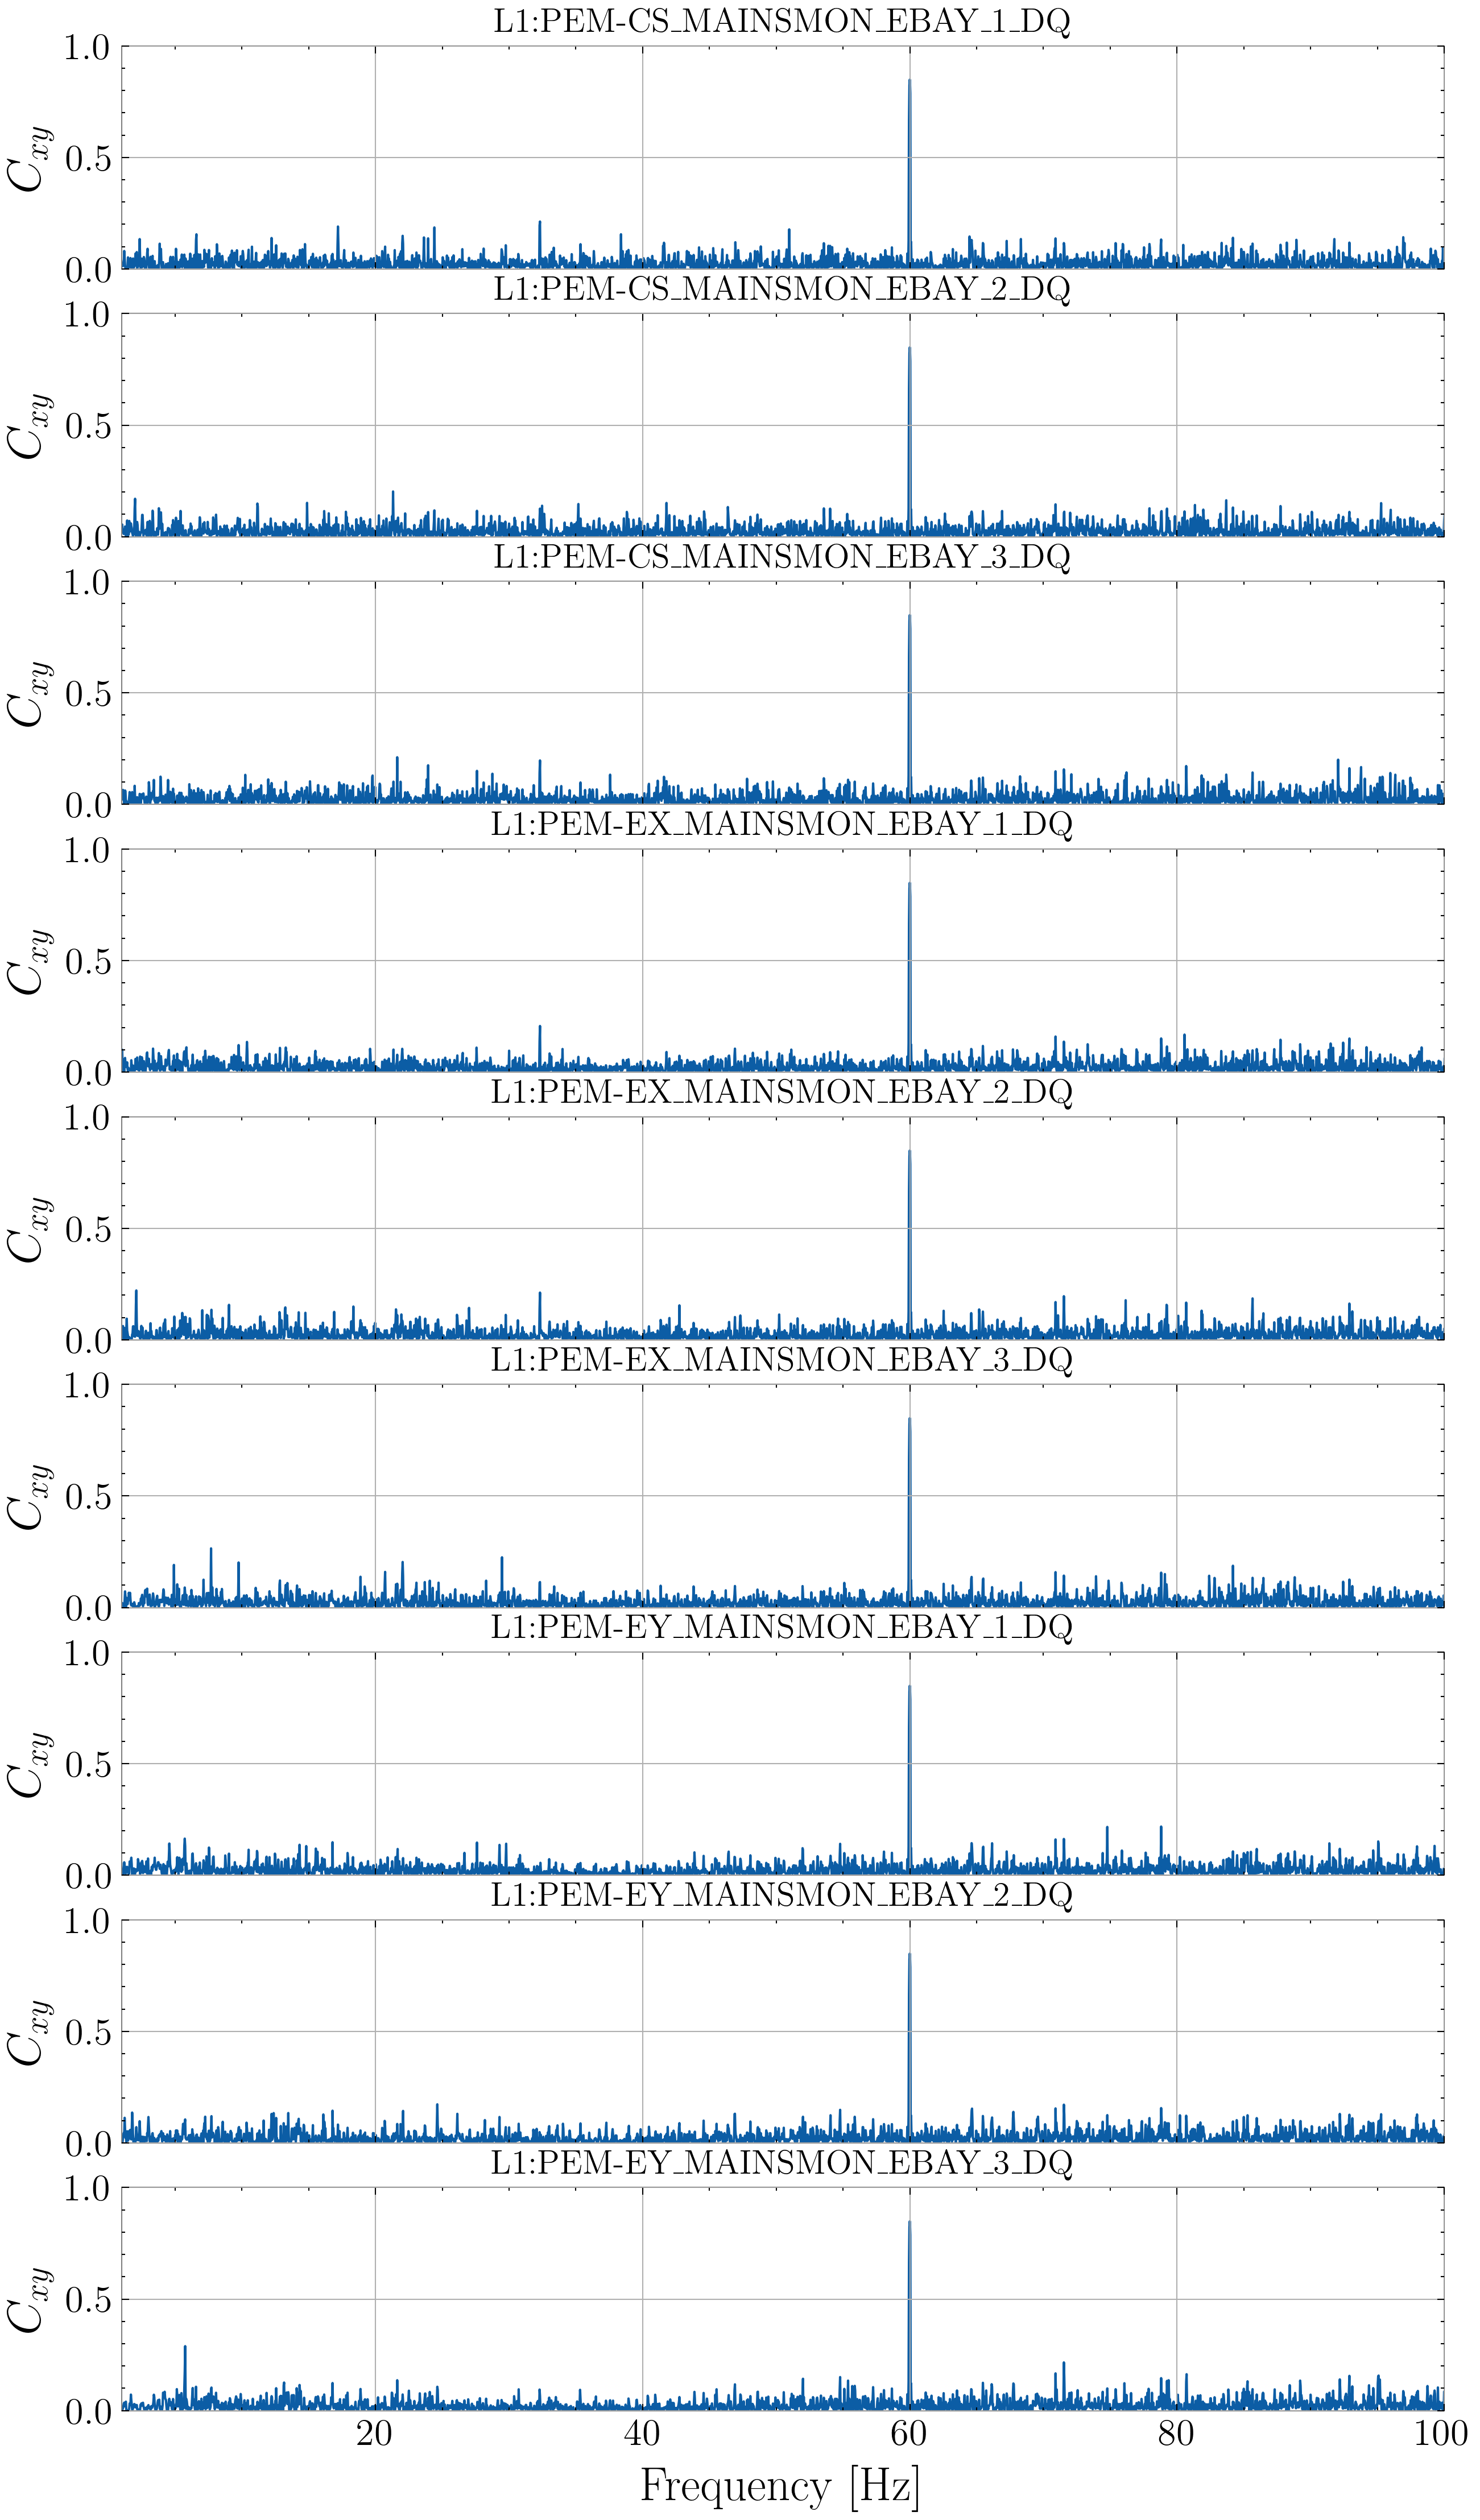
\includegraphics[width=\columnwidth]{images/stacked_coherence_plot}
	\end{center}
	\label{correlation_2}
	\caption{Coherence $C_{xy}$ between the LIGO-Livingston strain channel  \texttt{L1:DCS-CALIB\_STRAIN\_C01\_AR} and the 9 PEM channels over a 10 minute observation period. Clear features at 60 Hz are present in all of the channels. The coherence is weakest for those PEM channels which do not measure voltage directly, but instead are microphones the the LIGO vacuum equipment area.}
\end{figure}
\begin{figure*}
	\begin{center}
		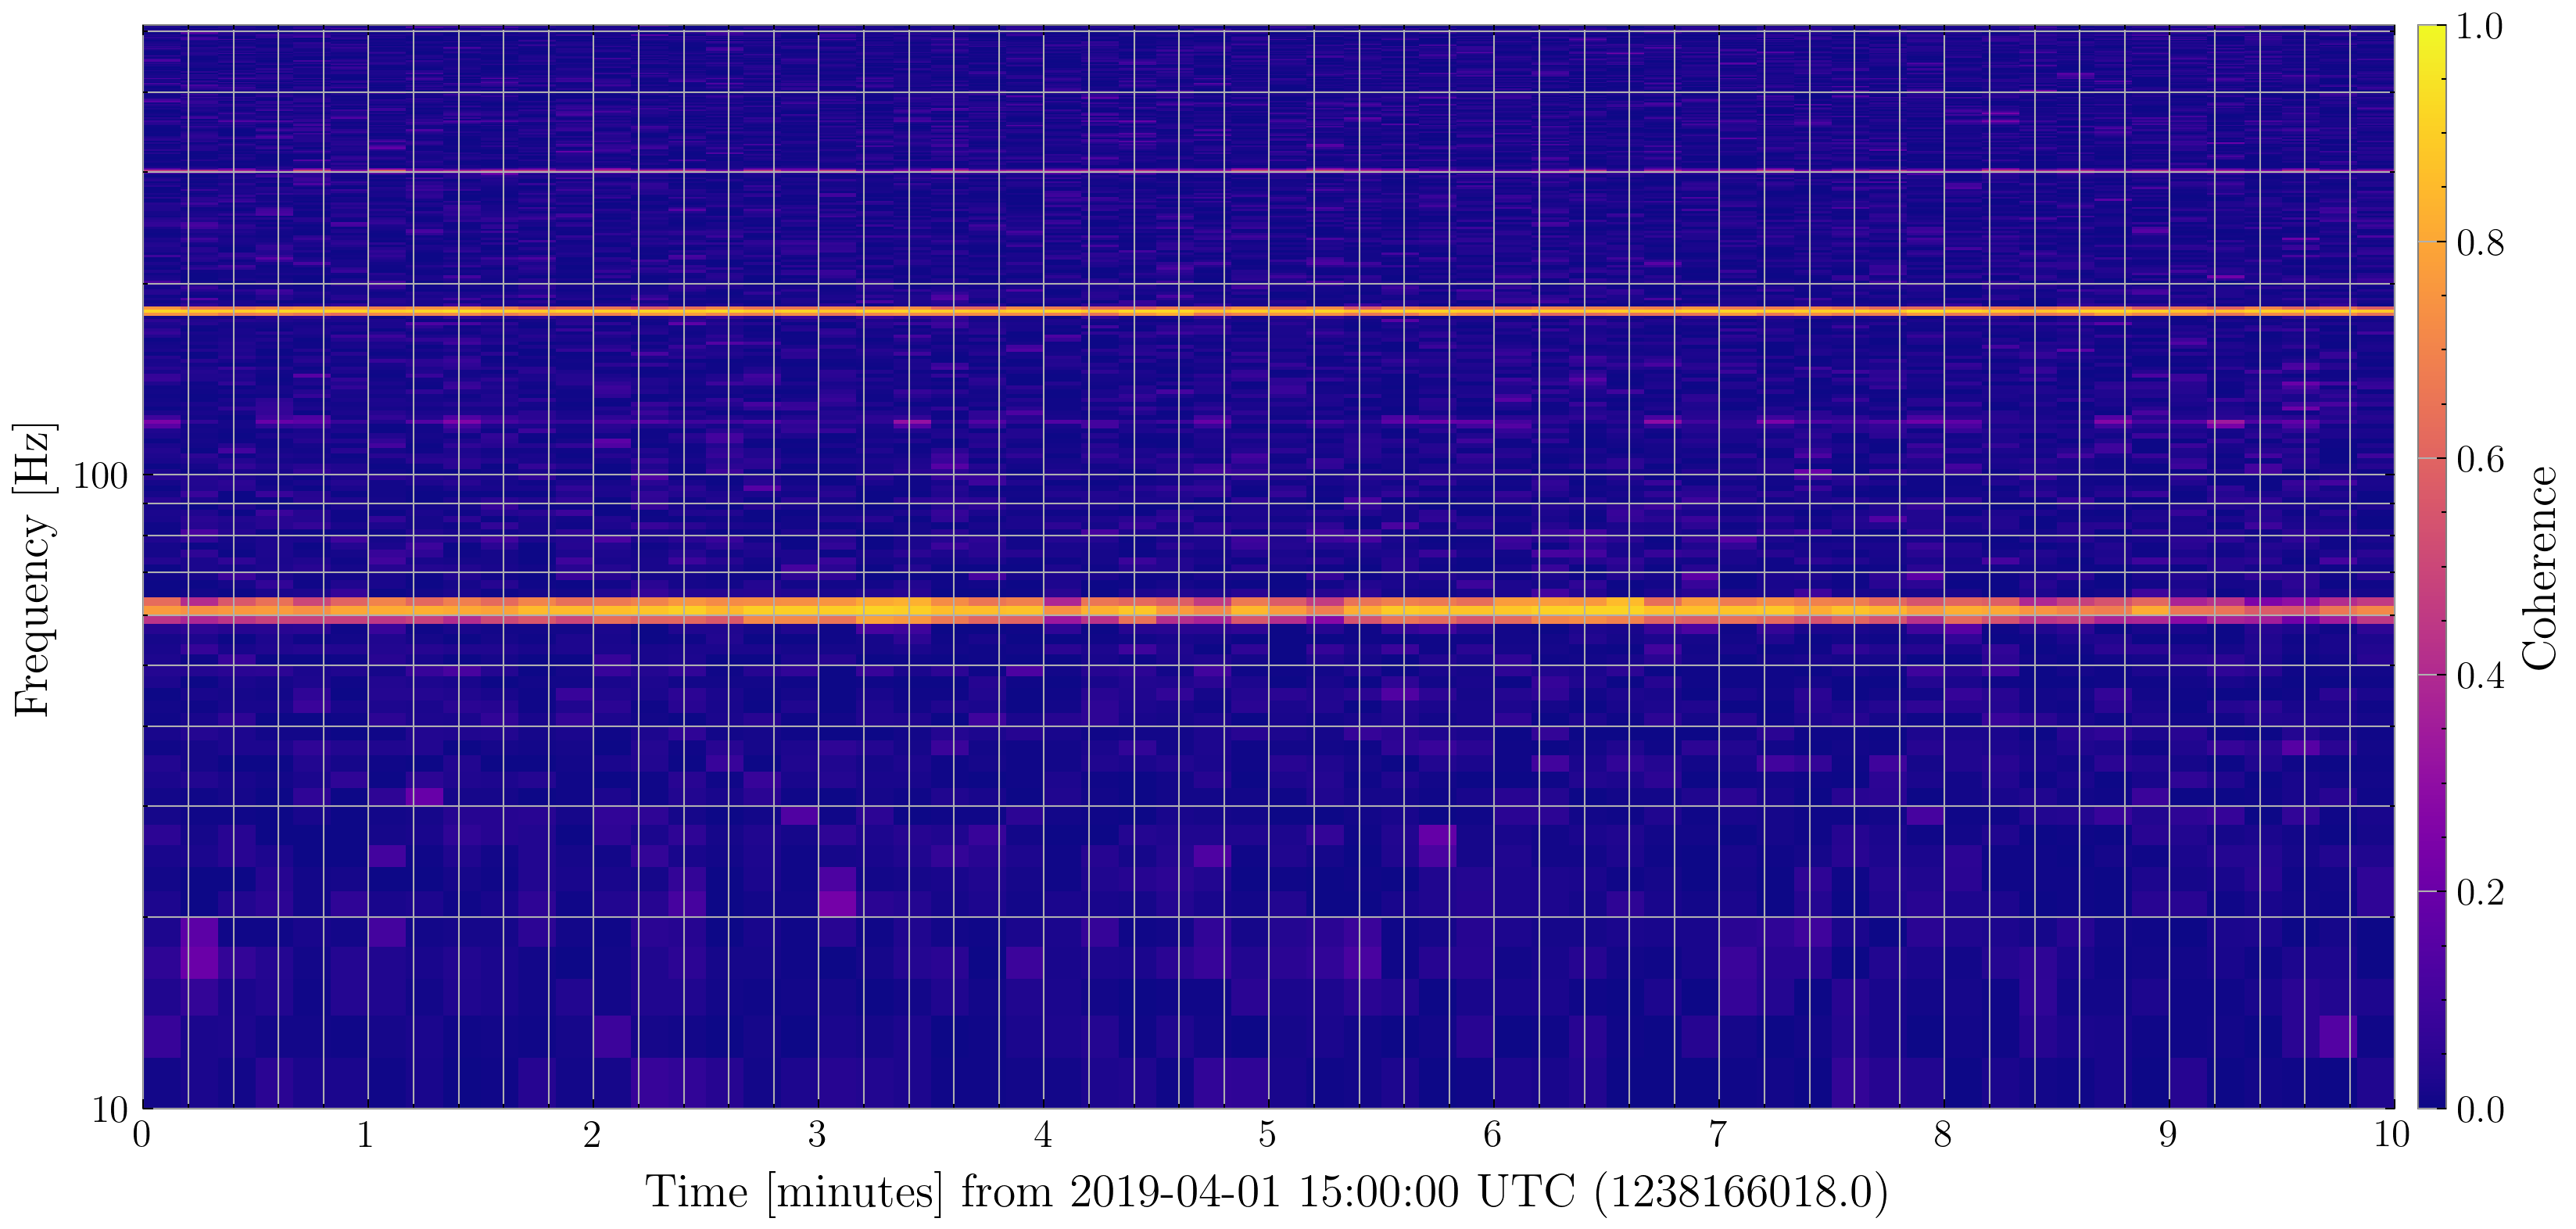
\includegraphics[width=\textwidth]{images/coherence_spectrogram}
	\end{center}
	\caption{\label{correlation_1}
		Coherence spectrogram between the strain channel \StrainChanName  and the PEM channel \PEMChanName  	over a 10 minute period of O3 data. A strong coherence is observed at 60Hz due to the main power interference. Additional coherence can also be observed at $\sim$ 200 Hz and 300 Hz due to instrumental lines of a different provenance c.f. Fig \ref{fig:strainSensitivity}.}
\end{figure*}



\section{Adaptive Noise Cancellation}\label{sec:method}


Adaptive Noise Cancellation (ANC) is a method for recovering an estimate of an underlying signal which has been corrupted or obscured by some additive noise interference \cite{Widrow1451965}. In contrast to other common optimal filtering methods (e.g. Wiener, Kalman) ANC requires no a-priori knowledge of either the signal or the noise. Instead, ANC makes use of a reference input which is correlated in some unknown way to the noise in the primary signal. This reference  can then be filtered and subtracted from the primary data series so as to recover the underlying signal. For our purposes, the primary timeseries is the gravitational-wave strain channel $x(t)$ (Equation \eqref{eq:data}) and the reference is a PEM recording voltage data from the power grid $r(t)$ (Equation \eqref{eq:voltage}). The objective of ANC is then to remove the clutter $c(t)$ of Equation \eqref{eq:data} with the aid of $r(t)$ whilst leaving $h(t)$ i.e. the signal of interest, intact. We now describe the ANC implementation used in this work. \newline 


The reference  $r(t)$ is used to construct an estimate of the clutter, $\hat{c}(t)$. The clutter estimate can then be subtracted from the primary signal in the time domain, defining a residual $e(t)$:
\begin{eqnarray}
	e(t) = x(t) - \hat{c}(t) \ .\label{eq:error_estimate}
\end{eqnarray}
As $\hat{c}(t) \to c(t)$, 	$e(t) \to h(t) + n(t)$ and we recover a noise cancelled timeseries. The clutter estimate is modelled by a finite duration impulse response (FIR) filter:
\begin{eqnarray}
	\hat{c}_k = \mathbf{w}^{\intercal}\mathbf{u}_k \ . \label{clutter_estimate}
\end{eqnarray}
where $\hat{c}_k$ is the clutter estimate at a discrete timestep $k$ (i.e. $\hat{c}_k = \hat{c}(t_{n_k})$), $\mathbf{u}_k$ is the tap-input vector composed of $M$ running samples of the reference signal arranged backwards in time:
 \begin{eqnarray}
 	\mathbf{u}_k &= [r_k, r_{k-1}, \dots, r_{k-M+1}] \ ,
 \end{eqnarray}
and $\mathbf{w}$ is the tap-weight vector:
 \begin{eqnarray}
	\mathbf{w} = [w_1, w_{2}, \dots, w_{M}] \ .
\end{eqnarray}
We want to determine the optimal tap weights $\mathbf{w}_{\rm opt}$, those which minimise the mean square error cost function:
\begin{eqnarray}
	\mathbf{w}_{\rm opt} = \arg \min \sum_{t=t_1}^{t=t_{N}} |e(t)|^2 \ .
\end{eqnarray}
This minimization problem can be solved by way of an adaptive recursive least squares (ARLS) method which we now describe in Section \ref{sec:ARLS}



\subsection{Adaptive Recursive Least Squares Method}
\label{sec:ARLS}
We now outline the ARLS method to compute the optimal tap weights and estimate the noise-subtracted signal. 
\begin{enumerate}
	\item Initialise the tap weights $\mathbf{w} = \mathbf{0}$ and a covariance matrix $\mathbf{P}= \delta^{-1} \mathbf{I}$, for regularisation parameter $0 < \delta \ll 1$  and identity matrix $\mathbf{I}$ of rank $M$.
	\item For $k=1, \dots, K$:
	
	\begin{enumerate}
		\item Estimate the clutter $\hat{c}_k$ by Equation \ref{clutter_estimate}
		\item Calculate the residual $e_k$ by Equation \ref{eq:error_estimate}
		\item Calculate the gain vector
		\begin{eqnarray}
			\mathbf{g}_k = \frac{\mathbf{P} \mathbf{u}_k}{\lambda + \mathbf{u}_k^{\intercal}\mathbf{P} \mathbf{u}_k}
		\end{eqnarray}
	\item Update the tap weights
			\begin{eqnarray}
		\mathbf{w} \mathrel{+}=  e_k \mathbf{g} 
	\end{eqnarray}
	\item Update the covariance matrix
\begin{eqnarray}
	\mathbf{P} \mathrel{+}= \lambda^{-1} \mathbf{P} - \mathbf{g} \lambda^{-1} \mathbf{P} \mathbf{u}_k^{\intercal} 
\end{eqnarray}

	\end{enumerate}

\end{enumerate}
The algorithm is also illustrated in Figure \ref{fig:arlsBlock} via a block diagram. \newline 


ARLS has two free parameters: the order parameter $M$ and the ``forgetting factor" $\lambda$, which is chosen so as to give exponentially less weight to older samples. The choice of $M$ influences the latency of the FIR filter, the computational overhead and the filter accuracy. In Sec.~\ref{sec:results} we trial a selection of $M$ values for synthetic GW data. The forgetting factor $\lambda$ ranges between 0 and 1, with $\lambda=1$ corresponding to infinite memory, causing the filter becomes an ordinary least squares method. In this work we use $\lambda=0.9999$. We refer the reader to Chapter 9 of Ref.~\cite{HaykinAdaptiveFT:2002} for a full review of adaptive least squares estimation in the context of linear filtering. 
\begin{figure}
	\begin{center}
		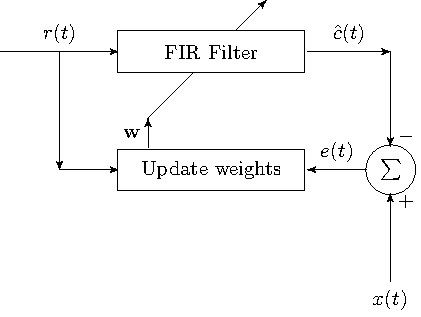
\includegraphics[width=\columnwidth]{images/FIR_block.pdf}
	\end{center}
	\caption{Block diagram of the adaptive recursive least squares method described in Section \ref{sec:ARLS}. The reference signal $r(t)$ is passed to an FIR filter to construct an estimate of the signal clutter $\hat{c}(t)$. Subtracting the clutter estimate from the primary signal $x(t)$ provides a residual $e(t)$ which can then be used to update the weights $\mathbf{w}$ of the FIR filter and the method proceeds iteratively.}
	\label{fig:arlsBlock}
\end{figure}

\section{HMM Validation tests} \label{sec:results}
We want to test the ANC method described in the preceding section by trying to search for a continuous wave signal which has an initial frequency $f_{\rm GW}(t=0) = 60 $Hz, coincident with the instrumental line from the mains power grid. We search for the CW signal using a HMM scheme based on the Viterbi algorithm \cite{Viterbi1,viterbi2}. Specifically, we use the method introduced by \citet{Suvorova2016PhRv}, which has been thoroughly tested through multiple LVK searches \cite{Piccinni2022,Riles2023,Wette2023}. We do not cover any details of the HMM scheme in this work and refer the reader to \citet{Suvorova2016PhRv} for further information. The GW signal is obscured in the data by the presence of the mains power instrumental line. The challenge is to try to recover the signal by first passing the data $x(t)$ through the ANC filter before using the HMM tracker on this filtered dataset to try to recover the signal. In Section \ref{sec:creating_data} we describe how we create a synthetic dataset $x(t)$. In Section \ref{sec:representative_example} we introduce a representative example, illustrating the frequency tracking before and after ANC. In Section \ref{sec:roc1} we explore the performance of the ANC filter in response to different characteristics of the interference signal, e.g. variations in the central frequency $f_{\rm ac}$ relative to the initial GW frequency. In Section \ref{sec:roc2} we investigate the performance of the filter in response to different filter settings; the order of the filter $M$ (i.e. the number of taps) and the number of reference channel inputs.

\subsection{Creating simulated data} \label{sec:creating_data}
Throughout this paper we work with some representative synthetic data, $x(t)$, rather than directly with the LIGO data itself. We can construct synthetic data for each of the constituent parts of Equation \eqref{eq:data} - the GW signal of interest, the Gaussian noise and the noise clutter via the formulation described in Section \ref{sec21} as follows. \newline 


The GW frequency evolves in general due to  the intrinsic evolution of the due to the intrinsic evolution of the source. For this paper  we assume that the source is isolated (i.e. it is not in a binary) and that the GW is monochromatic (i.e. all temporal derivatives of the frequency are zero). We also consider the GW source to be at a constant location with respect to the observer and neglect all contributions due to e.g. the rotation and revolution of the Earth. Under these assumptions the GW model reduces to 
\begin{equation}
	h(t) = h\sin(2\pi \phi_{\rm GW}(t)) \ , 
\end{equation}
where $h$ is the constant GW amplitude and $\phi(t)$ a random phase variable which is the integral of the underlying, piecewise linear GW frequency $f_{\rm gw}$ i.e.
\begin{equation}
	\phi_{\rm GW}(t) = \int_{0}^{t} f_{\rm gw}(s) ds \ .
\end{equation}
The GW frequency at discrete timestep $m$ within the sampling interval $\Delta t$ is labelled as $f_{\rm gw}^{(m)}$ and evolves according to
\begin{eqnarray}
	f_{\rm gw}^{(m+1)} = f_{\rm gw}^{(m)} + \delta_m \Delta t \ ,
\end{eqnarray}
with $\delta_m$ a zero mean Gaussian noise at timestep $m$, with variance $\sigma_f^2$,
\begin{equation}
	\delta_m = \mathcal{N}(0, \sigma_f^2) \label{eq:gwfreqnoise}
\end{equation}
The synthetic GW signal $h(t)$ is then completely described by the parameters $h$ and $\sigma_f^2$, and the initial GW frequency $f_{\rm gw}(t=0)$ \newline 


The clutter and reference signal evolve according to Equations \eqref{eq:voltage} and \eqref{eq:vclutter} respectively. For this initial study we take the reference voltage to have a constant amplitude $A_r(t) = a_r$, the clutter to have a corresponding constant amplitude $A_c(t) = a_c$. We also assume that the modulation in the reference voltage about $f_{\rm ac}$ has a constant amplitude $\Delta f_{\rm ac}$ with a constant period $P(t) = P$. Throughout this work we take $\Delta f_{\rm ac} = 1/2\pi$ Hz \footnote{\tiny \textcolor{red}{TK: I have guessed that this is what is happening under the hood of the code, but need to verify with Sofia/Changrong.}\normalsize}. We define the variable $\gamma = P^{-1}$ and explore different values for $\gamma$ in Section \ref{sec:roc1}. Under these assumptions, Equations \eqref{eq:voltage} and \eqref{eq:vclutter} reduce to 
\begin{align}
	r(t) = &a_r \cos \left[ 2 \pi f_{\rm ac} t + 2 \pi \cos\left(2 \pi \gamma t\right) + n_{\Theta} (t)\right] \\ \nonumber 
	&+n_r(t) \ ,
\end{align}
\begin{eqnarray}
	c(t) = &a_c \cos \left[ 2 \pi f_{\rm ac} t' + 2 \pi \cos\left(2 \pi \gamma t' \right) + n_{\Theta} (t')\right] \ .
\end{eqnarray}
The synthetic reference and clutter data are then completely described by the amplitude parameters $a_r,a_c$, the central frequency $f_{\rm ac}$, the timescale $\gamma$ and the noise covariances $\sigma^2_{\Theta}$, $\sigma_r^2$. For convenience we reparametrise $f_{\rm ac}$ relative to the initial GW frequency at $t=0$, defining the new variable
\begin{eqnarray}
	\Delta f = |f_{\rm ac} - f_{\rm gw}(t=0)|
\end{eqnarray}
The 9 free parameters of the model are summarised in Table \ref{tab:parameterdescription2}. We have 3 amplitude parameters $h, a_r, a_c$ for the GW, reference and clutter respectively, with $h \ll a_c, a_r$. There are 4 noise parameters $\sigma_n, \sigma_{\Theta}, \sigma_r, \sigma_f$ for the Gaussian noise $n(t)$, the voltage phase noise $n_{\Theta}(t)$, reference  signal measurement noise $n_r(t)$ and the GW frequency noise Equation \ref{eq:gwfreqnoise} respectively. Additionally we have the absolute difference between the central frequency and the initial GW frequency, $\Delta f$ and the timescale of the modulation in the central frequency,$\gamma$. \newline 



Throughout this work when creating synthetic data, $f_{\rm ac}$ is fixed at 60 Hz. The terrestrial noise parameters, $\sigma_n^2$,$\sigma_r^2$,$\sigma_{\Theta}^2$ are also fixed. \textcolor{red}{TK: other summary text on choice of parameters for synthetic data to go here. Waiting on input from Sofia on which parameters were actually used for the data}
\begin{table}[bp]
	
	\begin{tabular}{llc}
		\hline 
		
		Parameter & Physical meaning & Injected Value \\
		\hline
		$h$  &    Strain amplitude & - \\ 
		$a_r$ & Voltage amplitude &- \\
		$a_c$ & Clutter amplitude &- \\

		
		$\sigma_n^2$ & Gaussian noise covariance&- \\
		$\sigma_r^2$  & Voltage measurement noise & -\\
		$\sigma_{\Theta}^2$ & Voltage phase noise  &-\\
		$\sigma^2_f$ &  GW frequency noise & -\\
		
		$\Delta f$ &  Central frequency shift  &-\\
		$\gamma$ & Modulation frequency& - \\
		\hline
		
	\end{tabular} 
	
	\caption{Summary of parameters used to create synthetic data for testing the ANC method in Section \ref{sec:results}, their physical meaning, and the injected values used throughout this work.}
	\label{tab:parameterdescription2}
\end{table}



\subsection{Representative example} \label{sec:representative_example}
\begin{figure}
	\begin{center}
		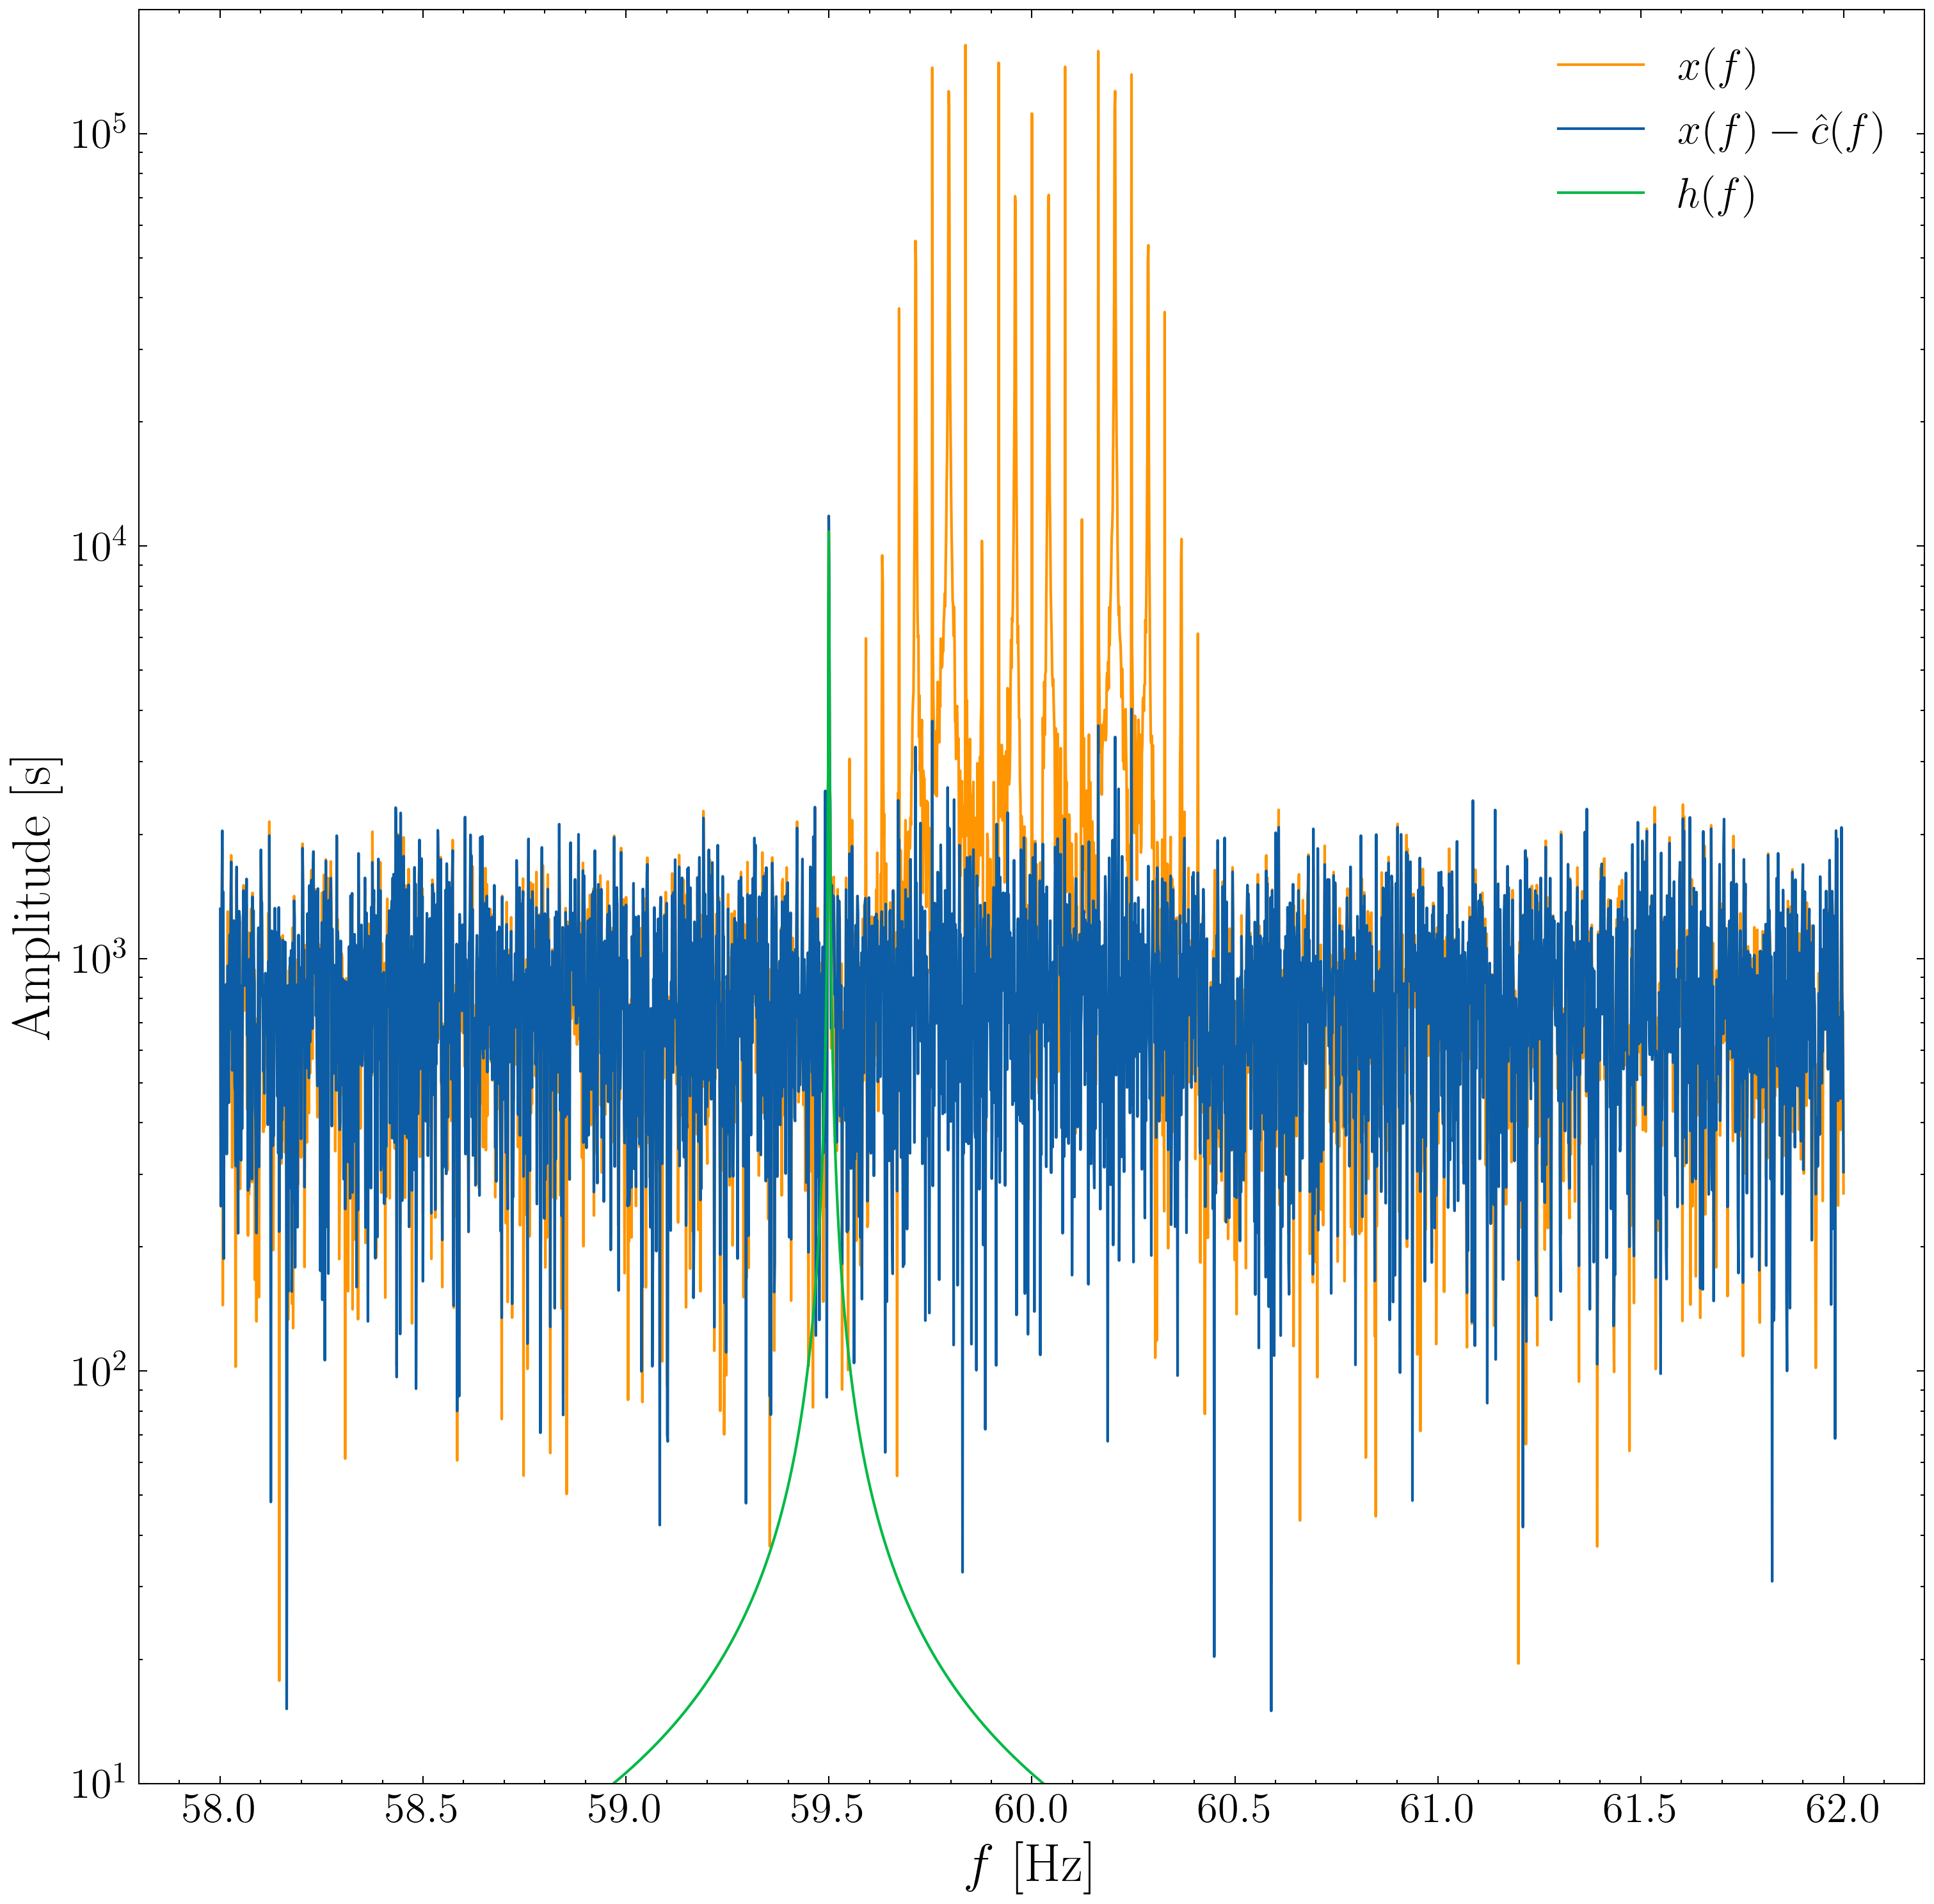
\includegraphics[width=\columnwidth]{images/spectrum.png}
	\end{center}
	\caption{Fourier response of the data $x(t)$ (orange), the GW signal $h(t)$ (green) and the ANC filtered data $x(t) - \hat{c}(t)$ (blue) for a system with parameters described in Table \ref{tab:parameterdescription2}. ANC filters out the excess power that results from the interference signal about the central 60 Hz frequency.}
	\label{fig:spectrum}
\end{figure}
\begin{figure*}
	\begin{center}
			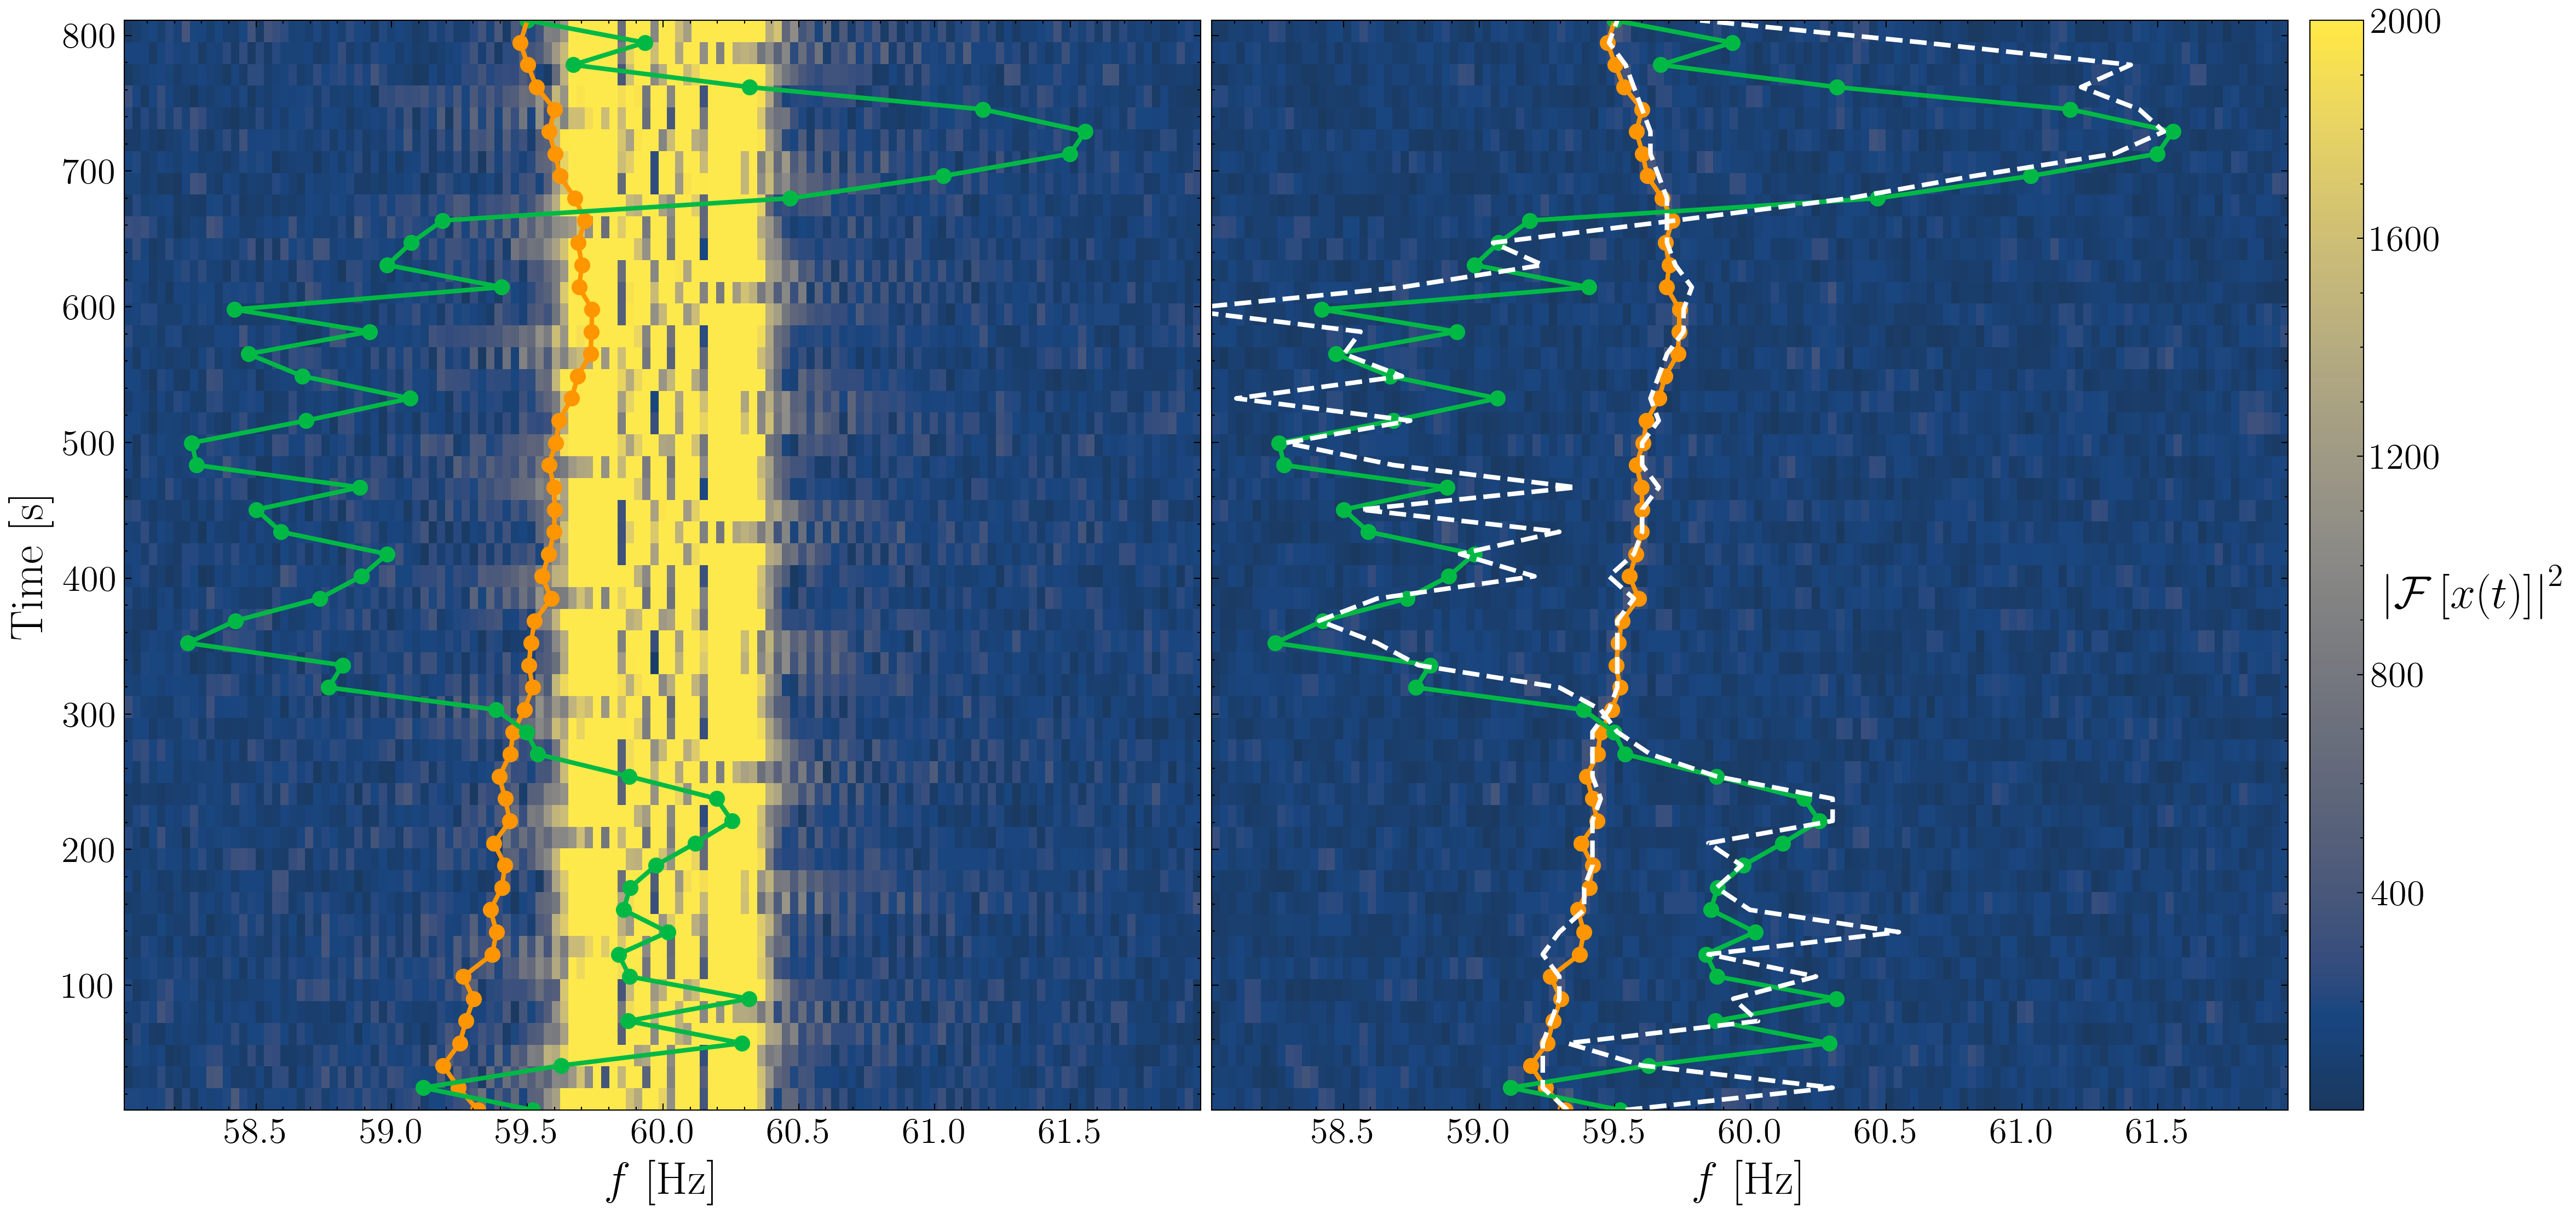
\includegraphics[width=\textwidth]{images/viterbi_tracking_canonical}
		\end{center}
	\caption{\label{frequency tracking before and after1}
			Fourier amplitude spectrogram and tracking of the frequency evolution of a continuous GW with $h = 0.025$ and $\sigma_f^2 = \{0.01, 0.1\}$ Hz $s^{-1/2}$ (orange and green lines respectively) using a HMM Viterbi algorithm. \textit{Left panel:}  before applying ANC filtering to remove the interference signal centred at 60Hz, \textit{Right panel:} after applying ANC. The Viterbi estimates of the spin wandering are noted by the dashed coloured lines. Before ANC, the Viterbi algorithm is unable to track the spin wandering. After ANC the Viterbi algorithm is able to track the GW frequency accurately for both the high and low noise cases.}
\end{figure*}

In order to demonstrate the effectiveness of ANC in conjunction with an HMM Viterbi search in this section we consider two representative examples where $h = 0.025$ and the stochastic GW frequency wandering is either `low', $\sigma_f^2 = 0.01$ Hz  $s^{-1/2}$ or `high', $\sigma_f^2 = 0.1$ Hz  $s^{-1/2}$. All other free parameters of the model are as specified in Table \ref{tab:parameterdescription2}. At this stage we assume that we have just one single reference PEM channel. \newline 


Initially we verify that the ANC filter works as expected to remove the excess power from the 60Hz interference. In Figure \ref{fig:spectrum} we show the Fourier amplitude of the synthetic data $x(t)$, the underlying GW signal $h(t)$, and the signal after being passed through the ANC filter, $e(t) = x(t) - \hat{c}(t)$ across the frequency range 58 - 62 Hz, for the case where $\sigma_f^2 = 0.01$ Hz. Before filtering the Fourier spectrum of $x(t)$ has multiple modes about the central 60 Hz frequency as a result of the interference clutter. This clutter obscures the power from the GW signal. After filtering, this excess power is removed and the Fourier spectrum of $e(t)$ is flat, with the exception of a clear feature coincident with the central frequency of the injected GW.  \newline 
 
Having established the ability of the ANC method to filter out the interference clutter given a reference signal, we can deploy the ANC in conjunction with the Viterbi HMM. We pass the ANC filtered data to the HMM and evaluate the performance of the HMM in tracking the spin-wandering continuous wave signal. The results are shown in  Figure \ref{frequency tracking before and after1} for the case of both low and high frequency wandering, for a single realisation of the noise. The figure shows the Fourier amplitude spectrogram of the data $x(t)$ before and after the application of ANC filtering. The spin wandering of the GW source (green/orange lines) and the Viterbi estimate (dashed orange/yellow lines) of the spin wandering is superimposed onto the spectrogram. In the low noise case the GW spin frequency wanders close to, but below, the 60Hz interference line. In the high noise case the GW spin frequency wanders much more strongly over a larger range of frequencies and crosses the interference line, presenting a more difficult challenge for the Viterbi tracking algorithm. Before ANC there is a clear feature in the Fourier spectrogram corresponding to the 60 Hz interference signal. In this case the Viterbi algorithm is unable to track the GW spin wandering frequency signal which is submerged with respect to the voltage interference at 60 Hz. Conversely,  the application of the ANC enables the interference to be removed without perturbing the gravitational wave signal. In this case the Viterbi algorithm is able to track the GW frequency wandering in both the low and high noise cases with high fidelity. Specifically, the mean squared error in the frequency estimate is $1.4 \times 10^{-3}$ Hz for the low noise case and $0.22$ Hz for the high noise case. 




\subsection{ROC curves versus power line parameters} \label{sec:roc1}

\begin{figure}
	\begin{center}
			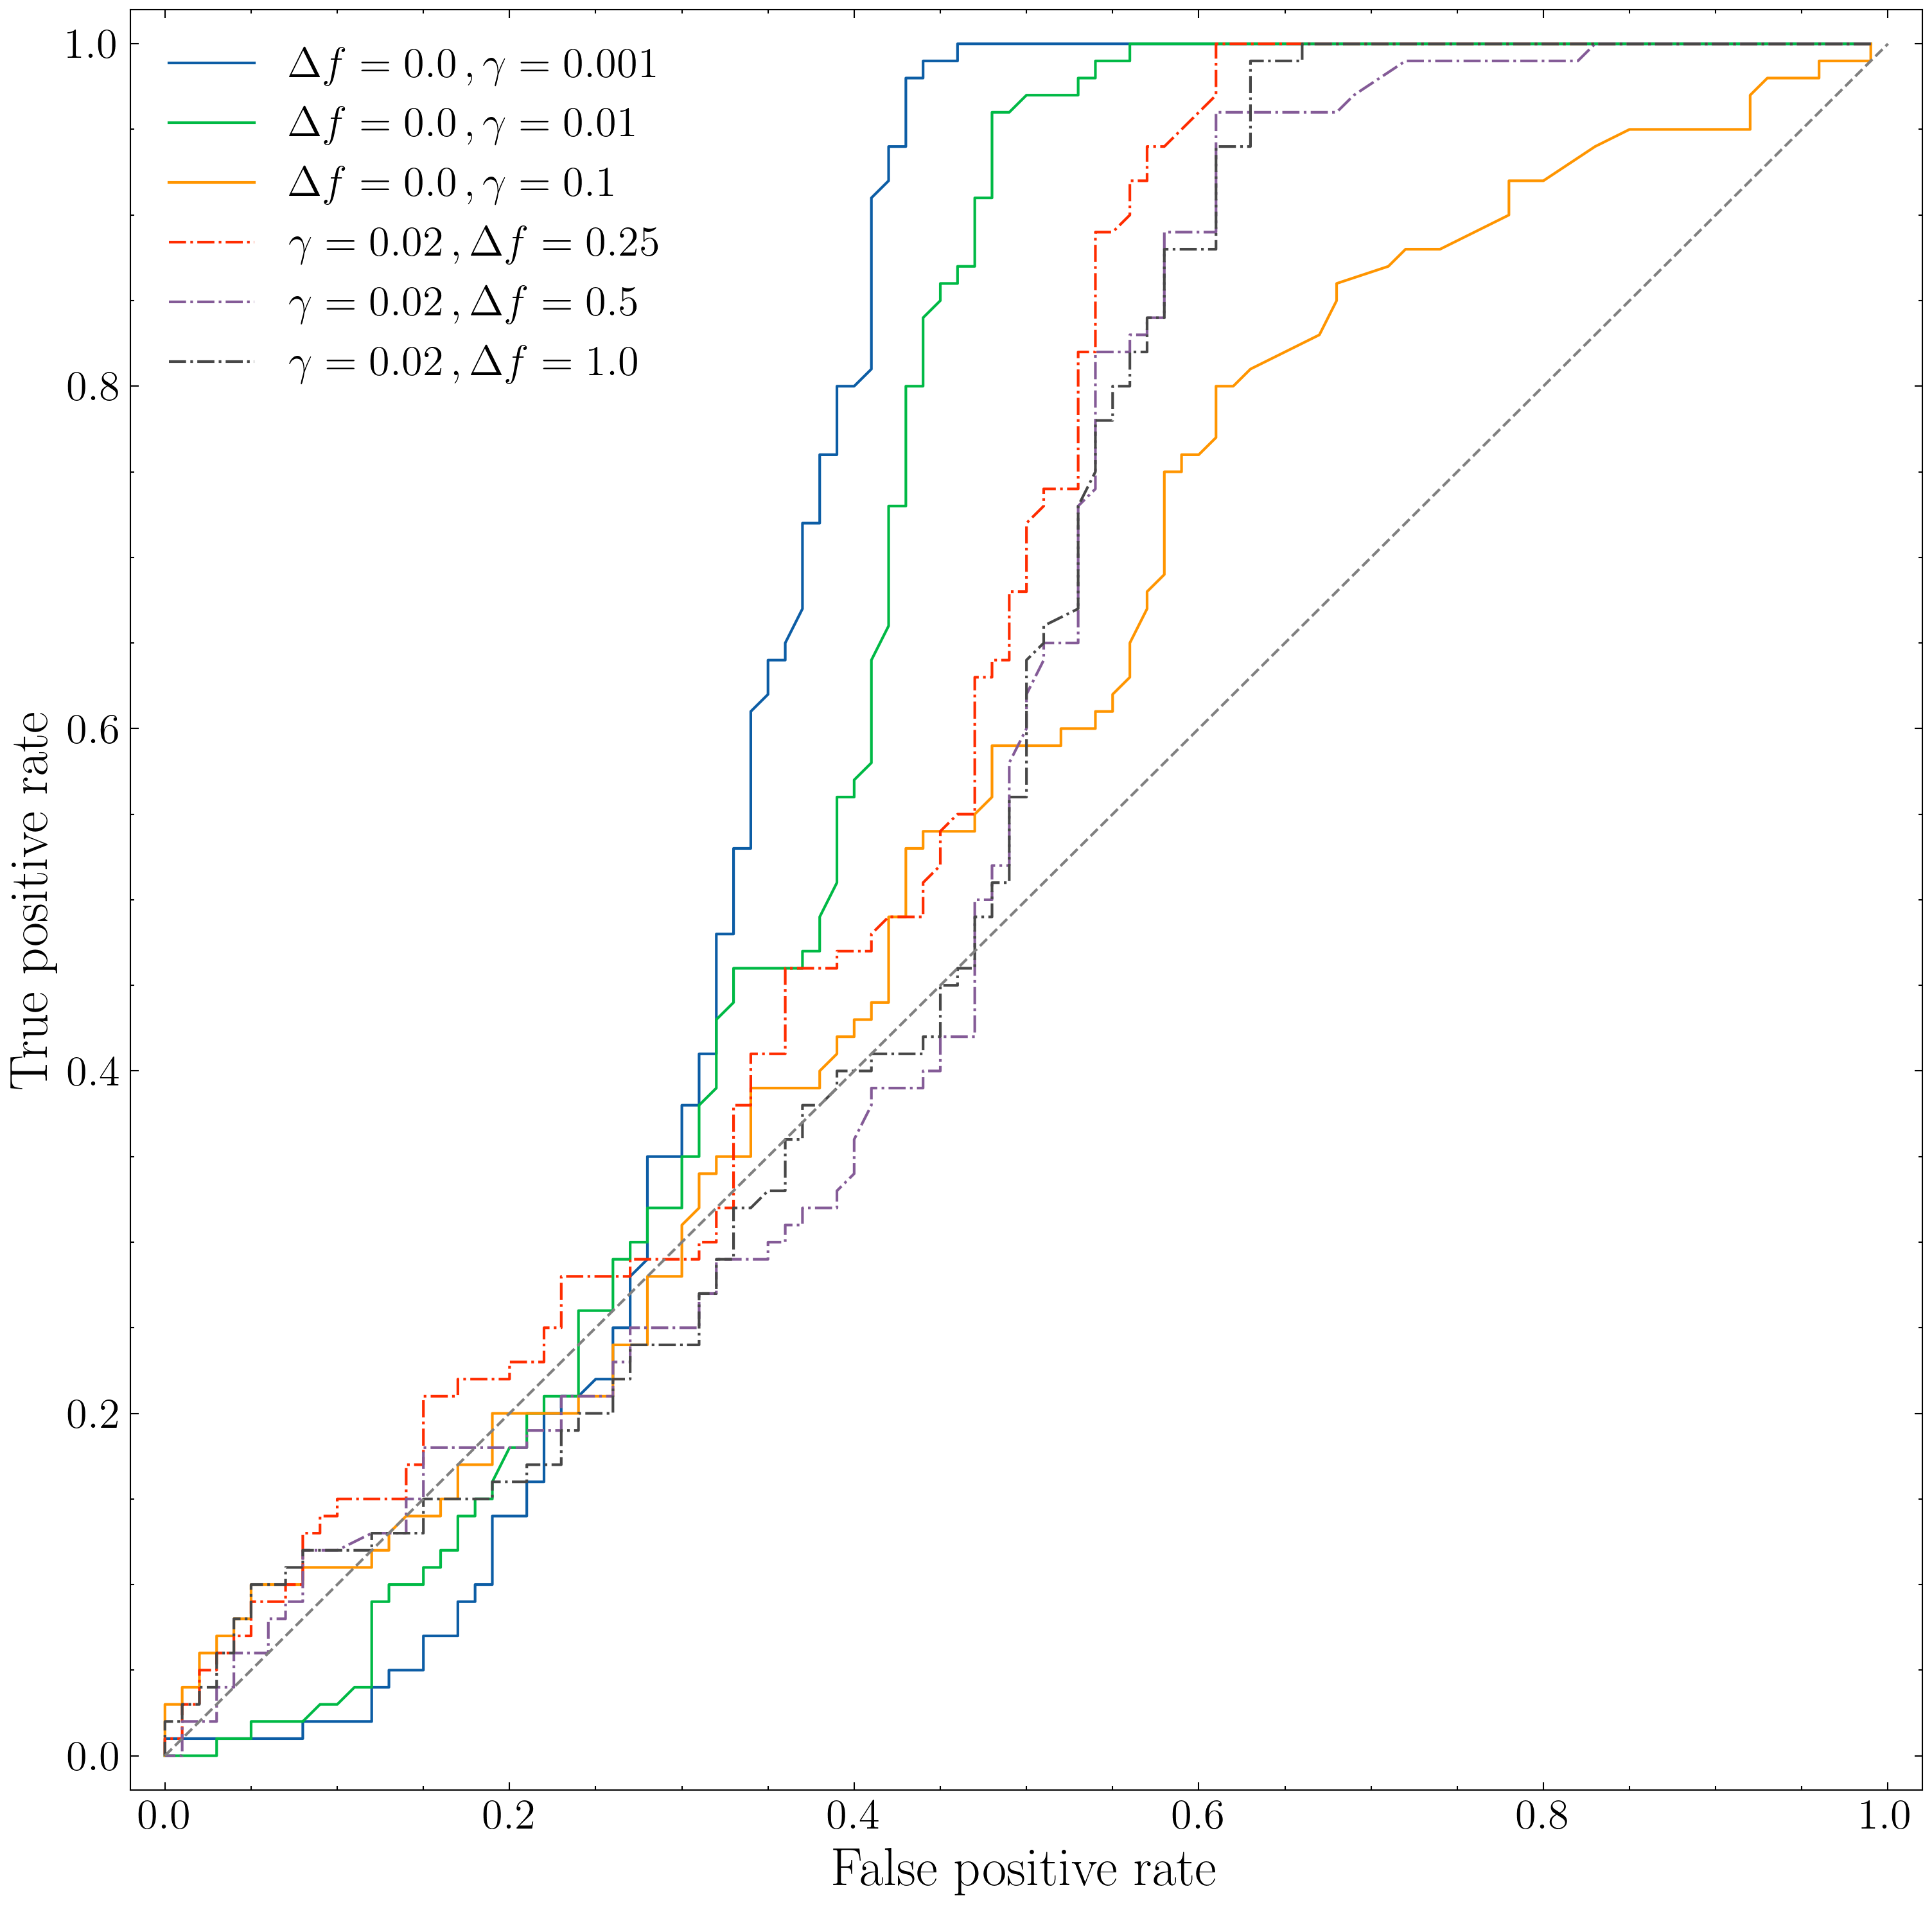
\includegraphics[width=\columnwidth]{images/4C_roccurve.png}
		\end{center}
	\caption{ROC curve over multiple noise realisations for different power line parameters. All other parameters are as specified in Table \ref{tab:parameterdescription2}. There is an evident high false alarm rate for all parameters, with a low AUC value of 0.55 for $\Delta f =0.0$, $\gamma=0.1$, and a high AUC value of 0.68 for $\Delta f =0.0$, $\gamma=0.001$. The high false alarm rate is a result of the interference not being completely removed by the ANC filter.}
	\label{fig:roc1}
\end{figure}
With the performance of the ANC and Viterbi approach established for a single example, it is of interest to explore how the algorithm performs for different power line parameters. In this section we vary $\Delta f$ and $\gamma$ to test how the combined ANC filter and Viterbi algorithm perform across multiple noise realisations. To this end we calculate the detection probability compared to the false alarm probability, i.e. the receiver operating characteristic (ROC), for the Viterbi search after the data has been filtered using ANC. We consider two situations. In the first situation we hold $\Delta f$ constant at $\Delta f =0.0$ and set $\gamma = \{ 0.001, 0.01, 0.1\}$. In the second situation we hold $\gamma$ constant at $\gamma = 0.02$ and set  $\Delta f = \{0.25, 0.5,1.0\}$. The results are shown in Figure \ref{fig:roc1}. Whilst the underlying wandering GW frequency signal can generally be tracked well for a single noise realisation (c.f. Figure \ref{frequency tracking before and after1}), we can see that for these power line parameters, across multiple noise realisations there is a high false alarm rate. This is a consequence of the interference not being completely removed and evidences how even a small quantity of clutter noise is sufficient to corrupt the search for continuous waves. To quantify the performance with a single scalar value we consider the Area Under the Curve (AUC), a common metric used to evaluate ROC curves. The AUC can be in the range $0.5 -- 1.0$, where $\text{AUC} = 0.5$ corresponds to the performance of a random classifier (i.e. the grey dashed diagonal line in the figure) and $\text{AUC} = 1.0$ represents a perfect classifier. For the first situation with $\Delta f =0.0$ and $\gamma = \{0.001, 0.01, 0.1\}$, AUC = $\{0.68, 0.65,0.55\}$ respectively. For the second situation with $\gamma = 0.02$ and $\Delta f = \{0.25, 0.5,1.0\}$, AUC = $\{0.62, 0.58,0.58\}$ respectively. Whilst the method performs better than a random classifier for all parameters, the AUC values are generally low, especially for cases where the interference has a large amplitude with a long period. In Section \ref{sec:roc2} we explore the use of different parameters used for the ANC filter, including the inclusion of additional reference channels




\subsection{ROC curves vs. filter parameters} \label{sec:roc2}
\begin{figure}
	\begin{center}
		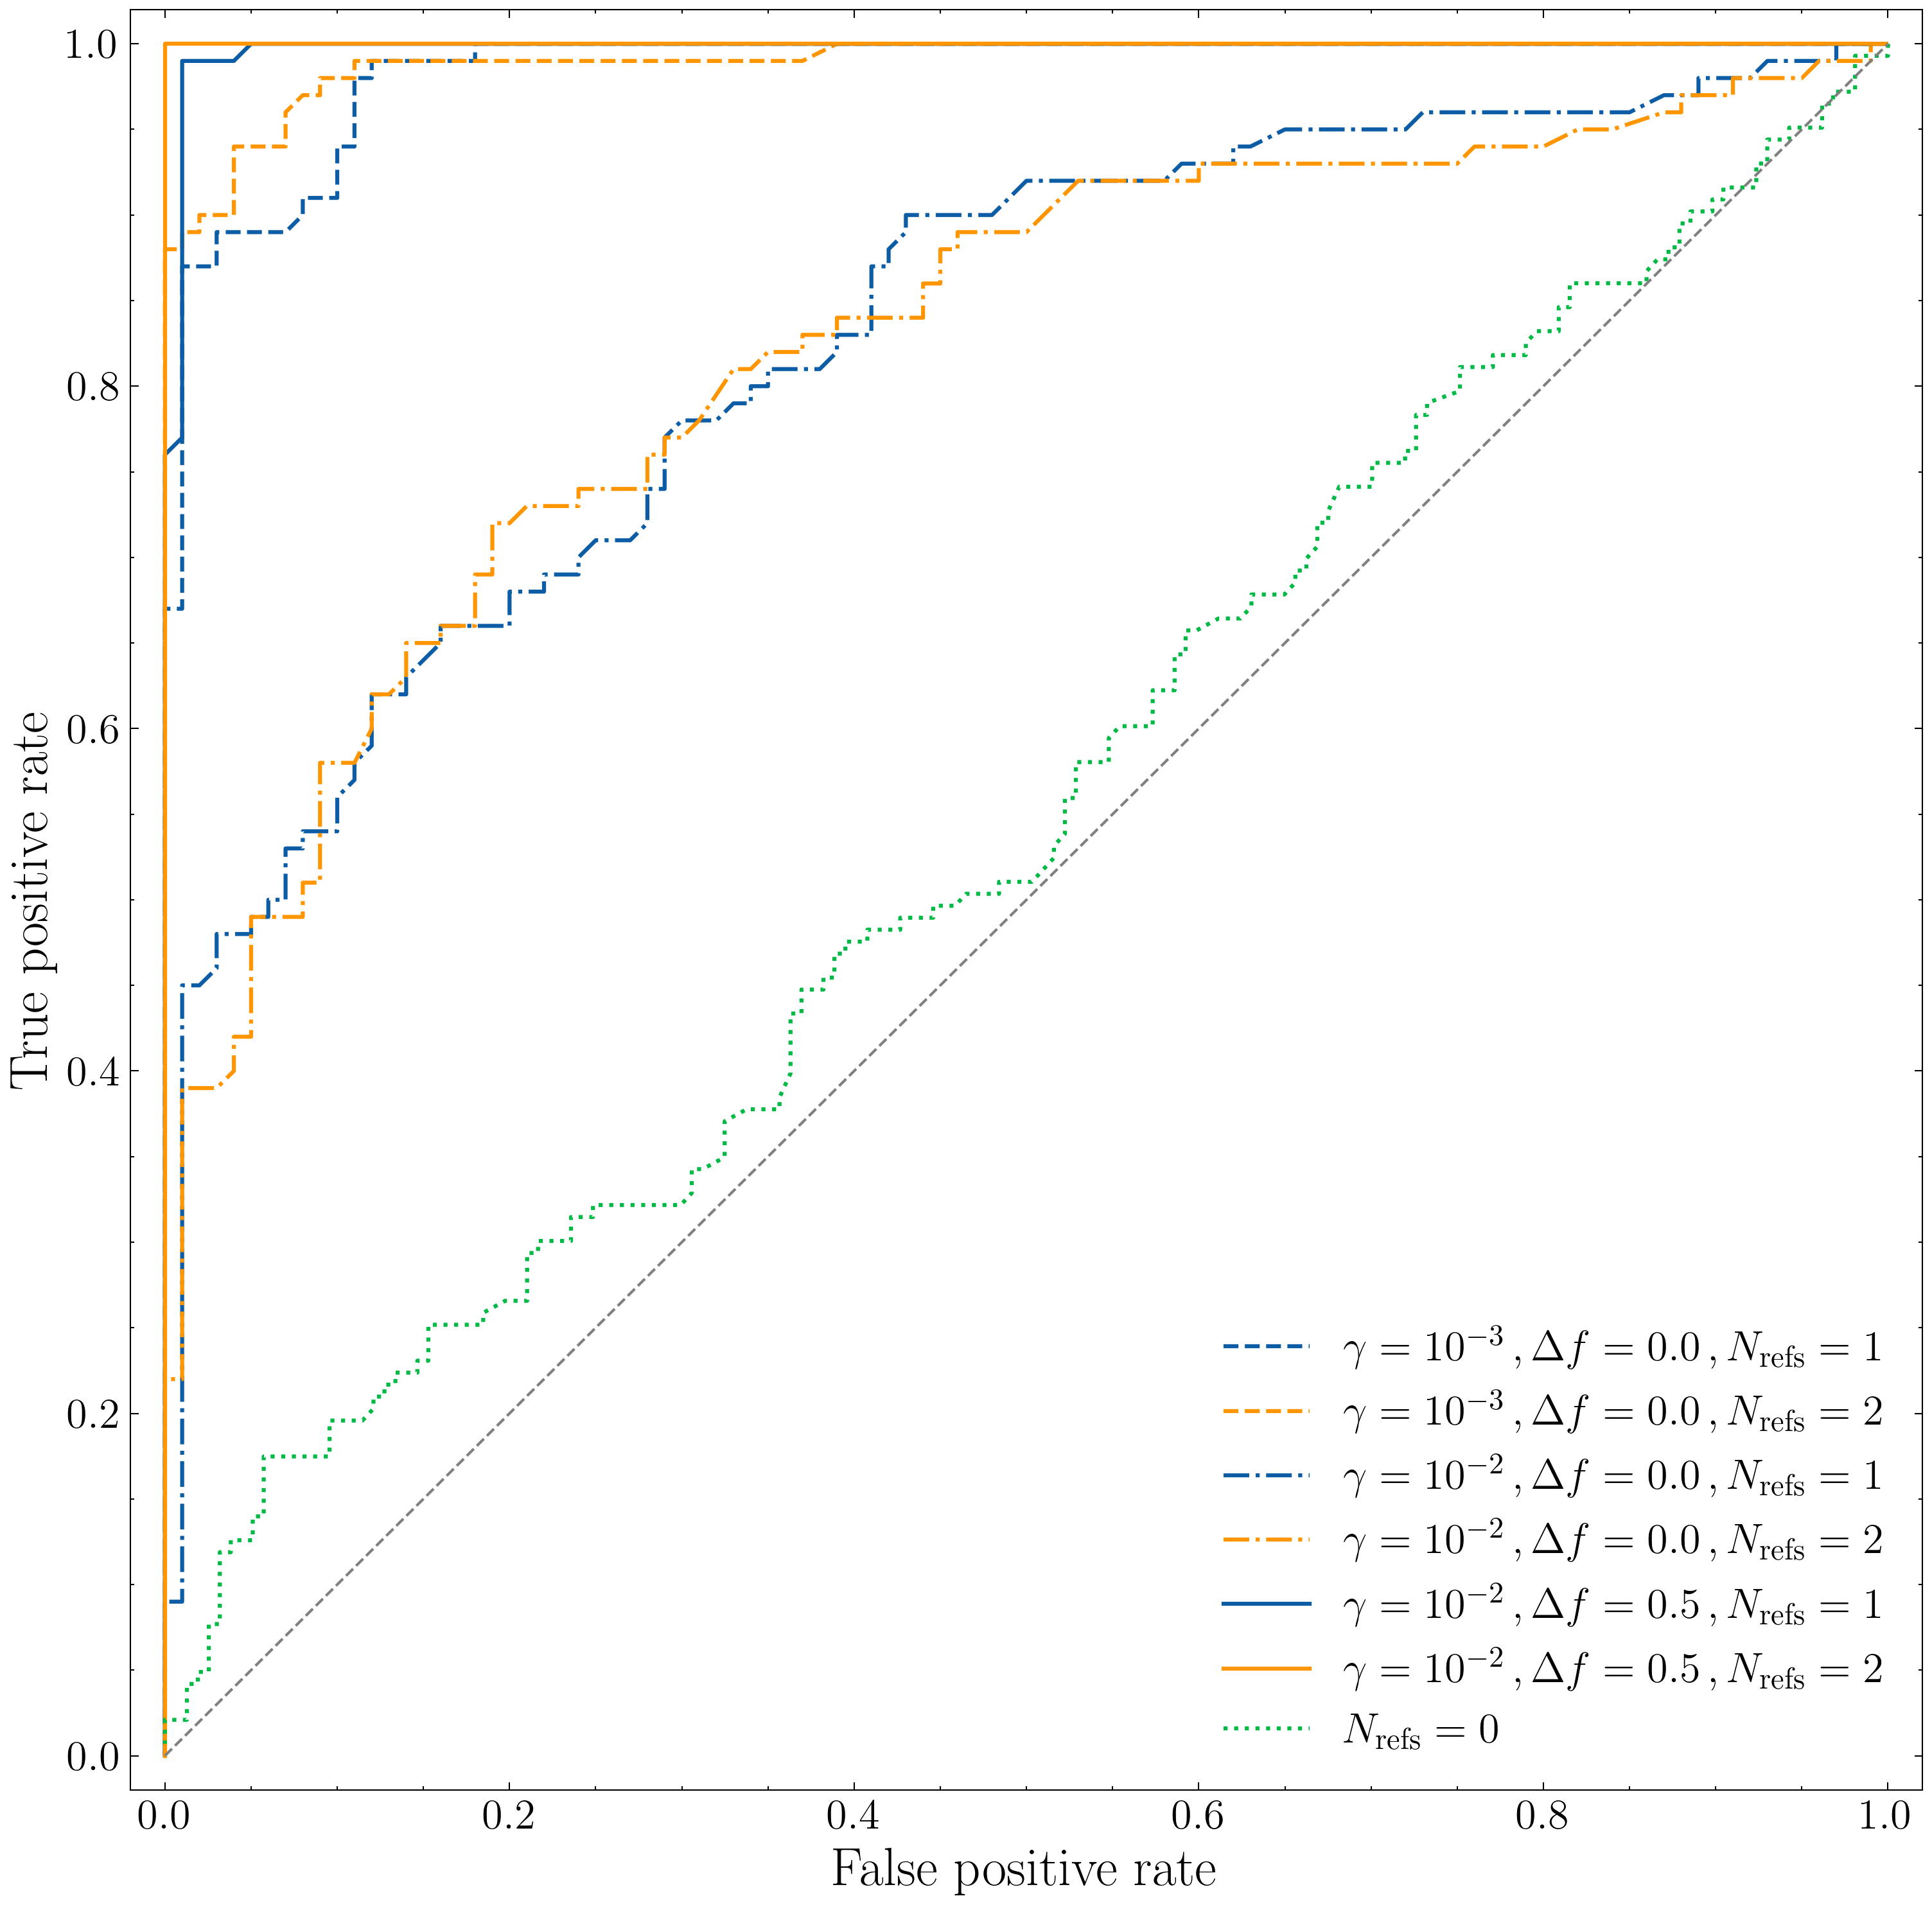
\includegraphics[width=\columnwidth]{images/4C_roccurve_multi_ref}
	\end{center}
	\caption{ROC curve for 3 different systems: System A with $\{ \gamma = 0.001, \Delta f = 0.0\}$, System B with $\{ \gamma = 0.01, \Delta f = 0.0\}$  and System C with $\{ \gamma = 0.01, \Delta f = 0.5\}$ (dotted, dashed, solid lines respectively). The orange lines denote the Viterbi search run with 2 reference channels, the blue lines using 1 reference channel. The green dotted line is the detection performance in the absence of ANC filtering. The grey dashed line is the performance of a random classifier. Detection using ANC filtering consistently outperforms that without ANC filtering. ANC filtering using 2 reference channels generally outperforms that using a single reference channel.}
	\label{fig:4C_roccurve_multi_ref}
\end{figure}
\begin{table}
	\centering
		\resizebox{0.4\columnwidth}{!}{%
		\begin{tabular}{l|ccc}
			\toprule
			\multicolumn{4}{c}{\hspace{6mm}System} \\
			
			$N_{\rm refs}$&A & B & C   \\
			\hline
			1& 0.975      & 0.827  & 0.987   \\
			2& 0.990         & 0.822   & 0.999  \\
			\bottomrule
		\end{tabular}
	}
		\caption{Summary of AUC values for each of the ROC curves presented in Figure \ref{fig:4C_roccurve_multi_ref}. Adding an extra PEM reference generally improves the detection performance, with the exception of system B. The AUC value for the zero PEM reference case (i.e. no ANC filtering) is $\text{AUC} = 0.55$.}
		\label{tab:AUC}
	\end{table}

\begin{figure}
	\begin{center}
		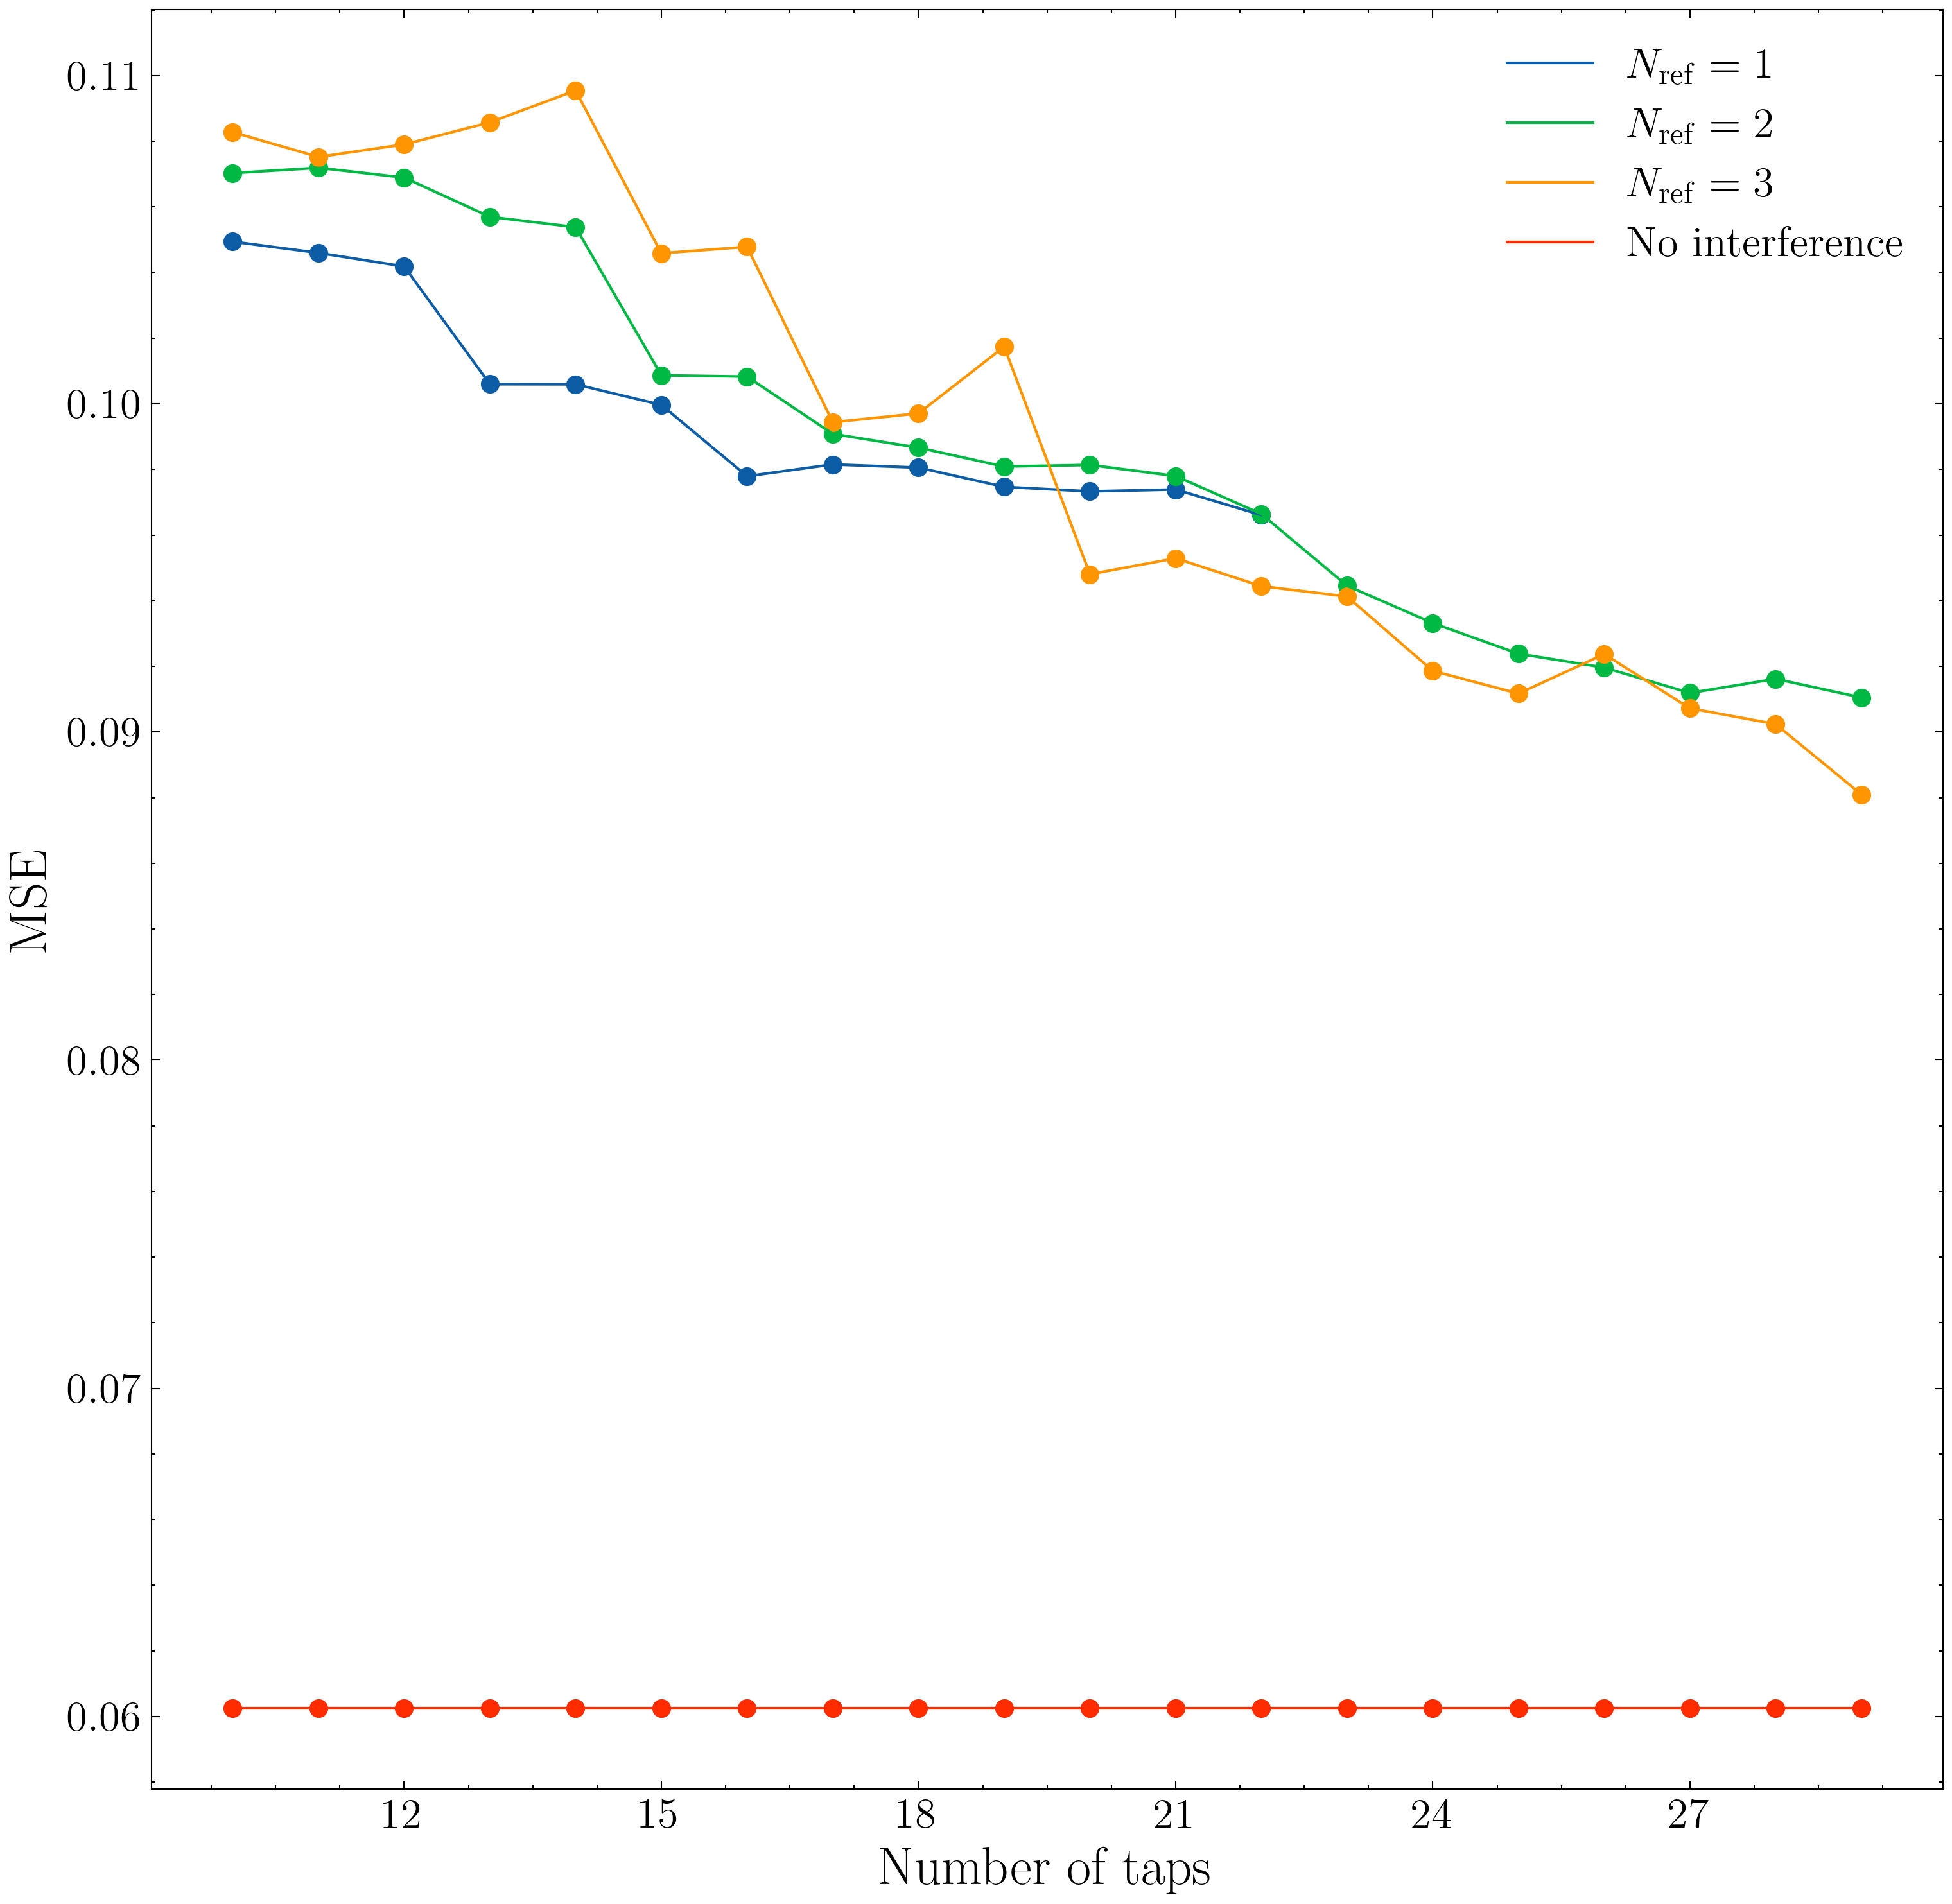
\includegraphics[width=\columnwidth]{images/taps_vs_error}
	\end{center}
	\caption{Mean square error (MSE) in the Viterbi estimates of the GW wandering spin frequency for a system with $h=0.025$ and $\Delta f =0.0$ relative to the number of taps used in the FIR filter. Up to three PEM reference channels are used. The solution for the case with zero interference clutter is also shown.}
	\label{fig:filterorder2}
\end{figure}


We have shown that the ANC filter used in conjunction with the Viterbi algorithm is effective at tracking the wandering GW spin frequency, but suffers from a high false alarm rate for the particular parameters of the ANC filter that we have been using. In this Section we investigate two important questions:
\begin{enumerate}
	\item How does ANC benefit from multiple independent references?
	\item What order ANC filter ($M$) is required to achieve good interference cancellation? 
\end{enumerate} 

Regarding the first question, the preceding validation tests on synthetic data all assumed that we have a single PEM reference voltage measurement. However, as discussed in Section \ref{sec23} in practice there are multiple PEM channels measuring power line interference for LIGO (c.f. Figure \ref{correlation_2}). Specifically, in the open O3a data there are 9 PEM channels for LIGO-Livingston and 7 PEM channels for LIGO-Hanford. Multiple PEM channels provided additional independent measurements of the reference voltage; it seems reasonable to suspect that these additional channels may aid the performance of the ANC filter. Indeed, ANC is commonly used with multiple reference signals in other electrical engineering applications such as noise cancelling headphones \citep{10.1121/1.5109394}, communication intelligibility \citep{KUO1996669,doi:10.1177/1084713812456906} and cardiac monitoring \citep{7755741}. \newline 

In Figure \ref{fig:4C_roccurve_multi_ref} we present the ROC curves for 3 different example systems:
\begin{itemize}
	\item \textbf{System A}. $\gamma = 10^{-3} \, , \Delta f = 0.0$. Dashed lines in the figure.
	\item \textbf{System B}. $\gamma = 10^{-2} \, , \Delta f = 0.0$. Dash-dotted in the figure
	\item \textbf{System C}. $\gamma = 10^{-2} \, , \Delta f = 0.5$. Solid lines in the figure
\end{itemize}
For each system we compute the ROC curve over multiple noise realisations for both one and two reference channels (blue, and orange lines respectively). This gives us six total ROC curve solutions. For comparison we also plot the case where we run the Viterbi search for one of the example systems, but with zero PEM references (dotted green line). The specific AUC values for each ROC curve are reported in Table \ref{tab:AUC}. \newline 

We can see that for all example systems the detection probability is high with respect to the false alarm probability. The detection probability using ANC filtering is greater than without ANC filtering for all systems (i.e. the orange and blue lines are exclusively above the green dotted line). Specifically the for the zero filtering case AUC$=0.54$, whilst all cases which use ANC filtering have AUC$\ge 0.82$ and as high as AUC$=0.99$. The inclusion of an additional reference channel improves the detection probability for Systems A and C, with the AUC values rising from 0.975 to 0.990 for System A and from $0.987$ to $0.999$ for System B. No improvement is observed for System B, with AUC$=0.827$ for $N_{\rm ref} =1$ and AUC$=0.822$ for $N_{\rm ref} =2$. The lack of improvement for System B when using two PEM references suggests that for these parameters a single reference is sufficient to capture the dynamics of the interference clutter. \newline  \footnote{\tiny \textcolor{red}{TK: Why are these results so different to Figure 8? Has the strain amplitude changed? Need to check with Sofia}\normalsize}

Regarding the second question, the order of the filter, i.e. the number of taps, is a parameter that can be freely chosen in ARLS. It is important to consider the filter's robustness to the choice of $M$. Generally an increased number of taps is expected to improve the performance of the filter due to the increased model complexity. However, this comes at an increased computational cost and also an increased latency. For real time applications tracking the wandering of the GW frequency it is important to minimize both of these variables. In Figure  \ref{fig:filterorder2} we plot the mean squared error (MSE) in the GW frequency estimated by Viterbi compared to the true spin-wandering frequency, averaged over multiple noise realisations. We set the system to have $h=0.025$ and $\Delta f =0.0$ and consider up to three PEM reference channels. As a reference we also plot the error in the Viterbi estimates for the case where there is no interference clutter and so no ANC is required. We can see that generally the accuracy improves with an increased number of taps. When $M$ is small the $N_{\rm ref} =1$ solution generally outperforms the high $N_{\rm ref}$ solutions; in this regime the number of taps is sufficiently small to not be able to take advantage of the increased information provided by the additional reference channels. Conversely as the number of taps increases, the $N_{\rm ref} =3$ becomes the best performing solution. We note that rather than explicitly specifying the number of taps, adaptive tap length methods that automatically update the number of taps used are also available \citep[e.g.][]{1326385,KAR2017422,KAR2020107043}.



%\begin{equation}
%	{\rm MSE}=E_{\rm emp} \left [(\sum_{i=0}^{KN}e_i^2)/(KN+1) \right ]
%\end{equation}
%where we use $E_{\rm emp} [X]$ to denote the empirical mean of a quantity $X$ over 500 simulations. \textcolor{red}{TK: confirm this equations is correct and what are K/N in the updated notation?}. The MSE as a function of the number of taps $M$ is shown in Fig \ref{mse vs tap} for a system with $|H(w)|=3$ and $\rm{SNR}_{\rm in}=0.02$. We can see that initially as the number of taps increases from the MSE deceases, finidng a minimum at around $M=64$. This is due to the narrower bandwidth enabling a sharper filter to remove more of the interference. Beyond this point the MSE starts to increase. Now the increased sharpness of the filter is hampered by the time delay from using too many taps and the filter is not able to track the frequency with a sufficiently small latency. 

%With the performance of the ANC and Viterbi approach established for a single example, it is of interest to explore how the algorithm performs for different power line parameters. In this section we vary $\Delta f$ and $\gamma$ to test the ANC and Viterbi performance for multiple noise realisations. To this end we calculate the detection probability compared to the false alarm probability, i.e. the receiver operating characteristic (ROC), for the Viterbi search after ANC. 
%
%
%In this paper we address two important questions 
%
%
%We investigate this by computing the 
%mean square difference between the signal after applying the ANC with the signal without interference as function of the order. 


%\begin{figure}
%	\begin{center}
%		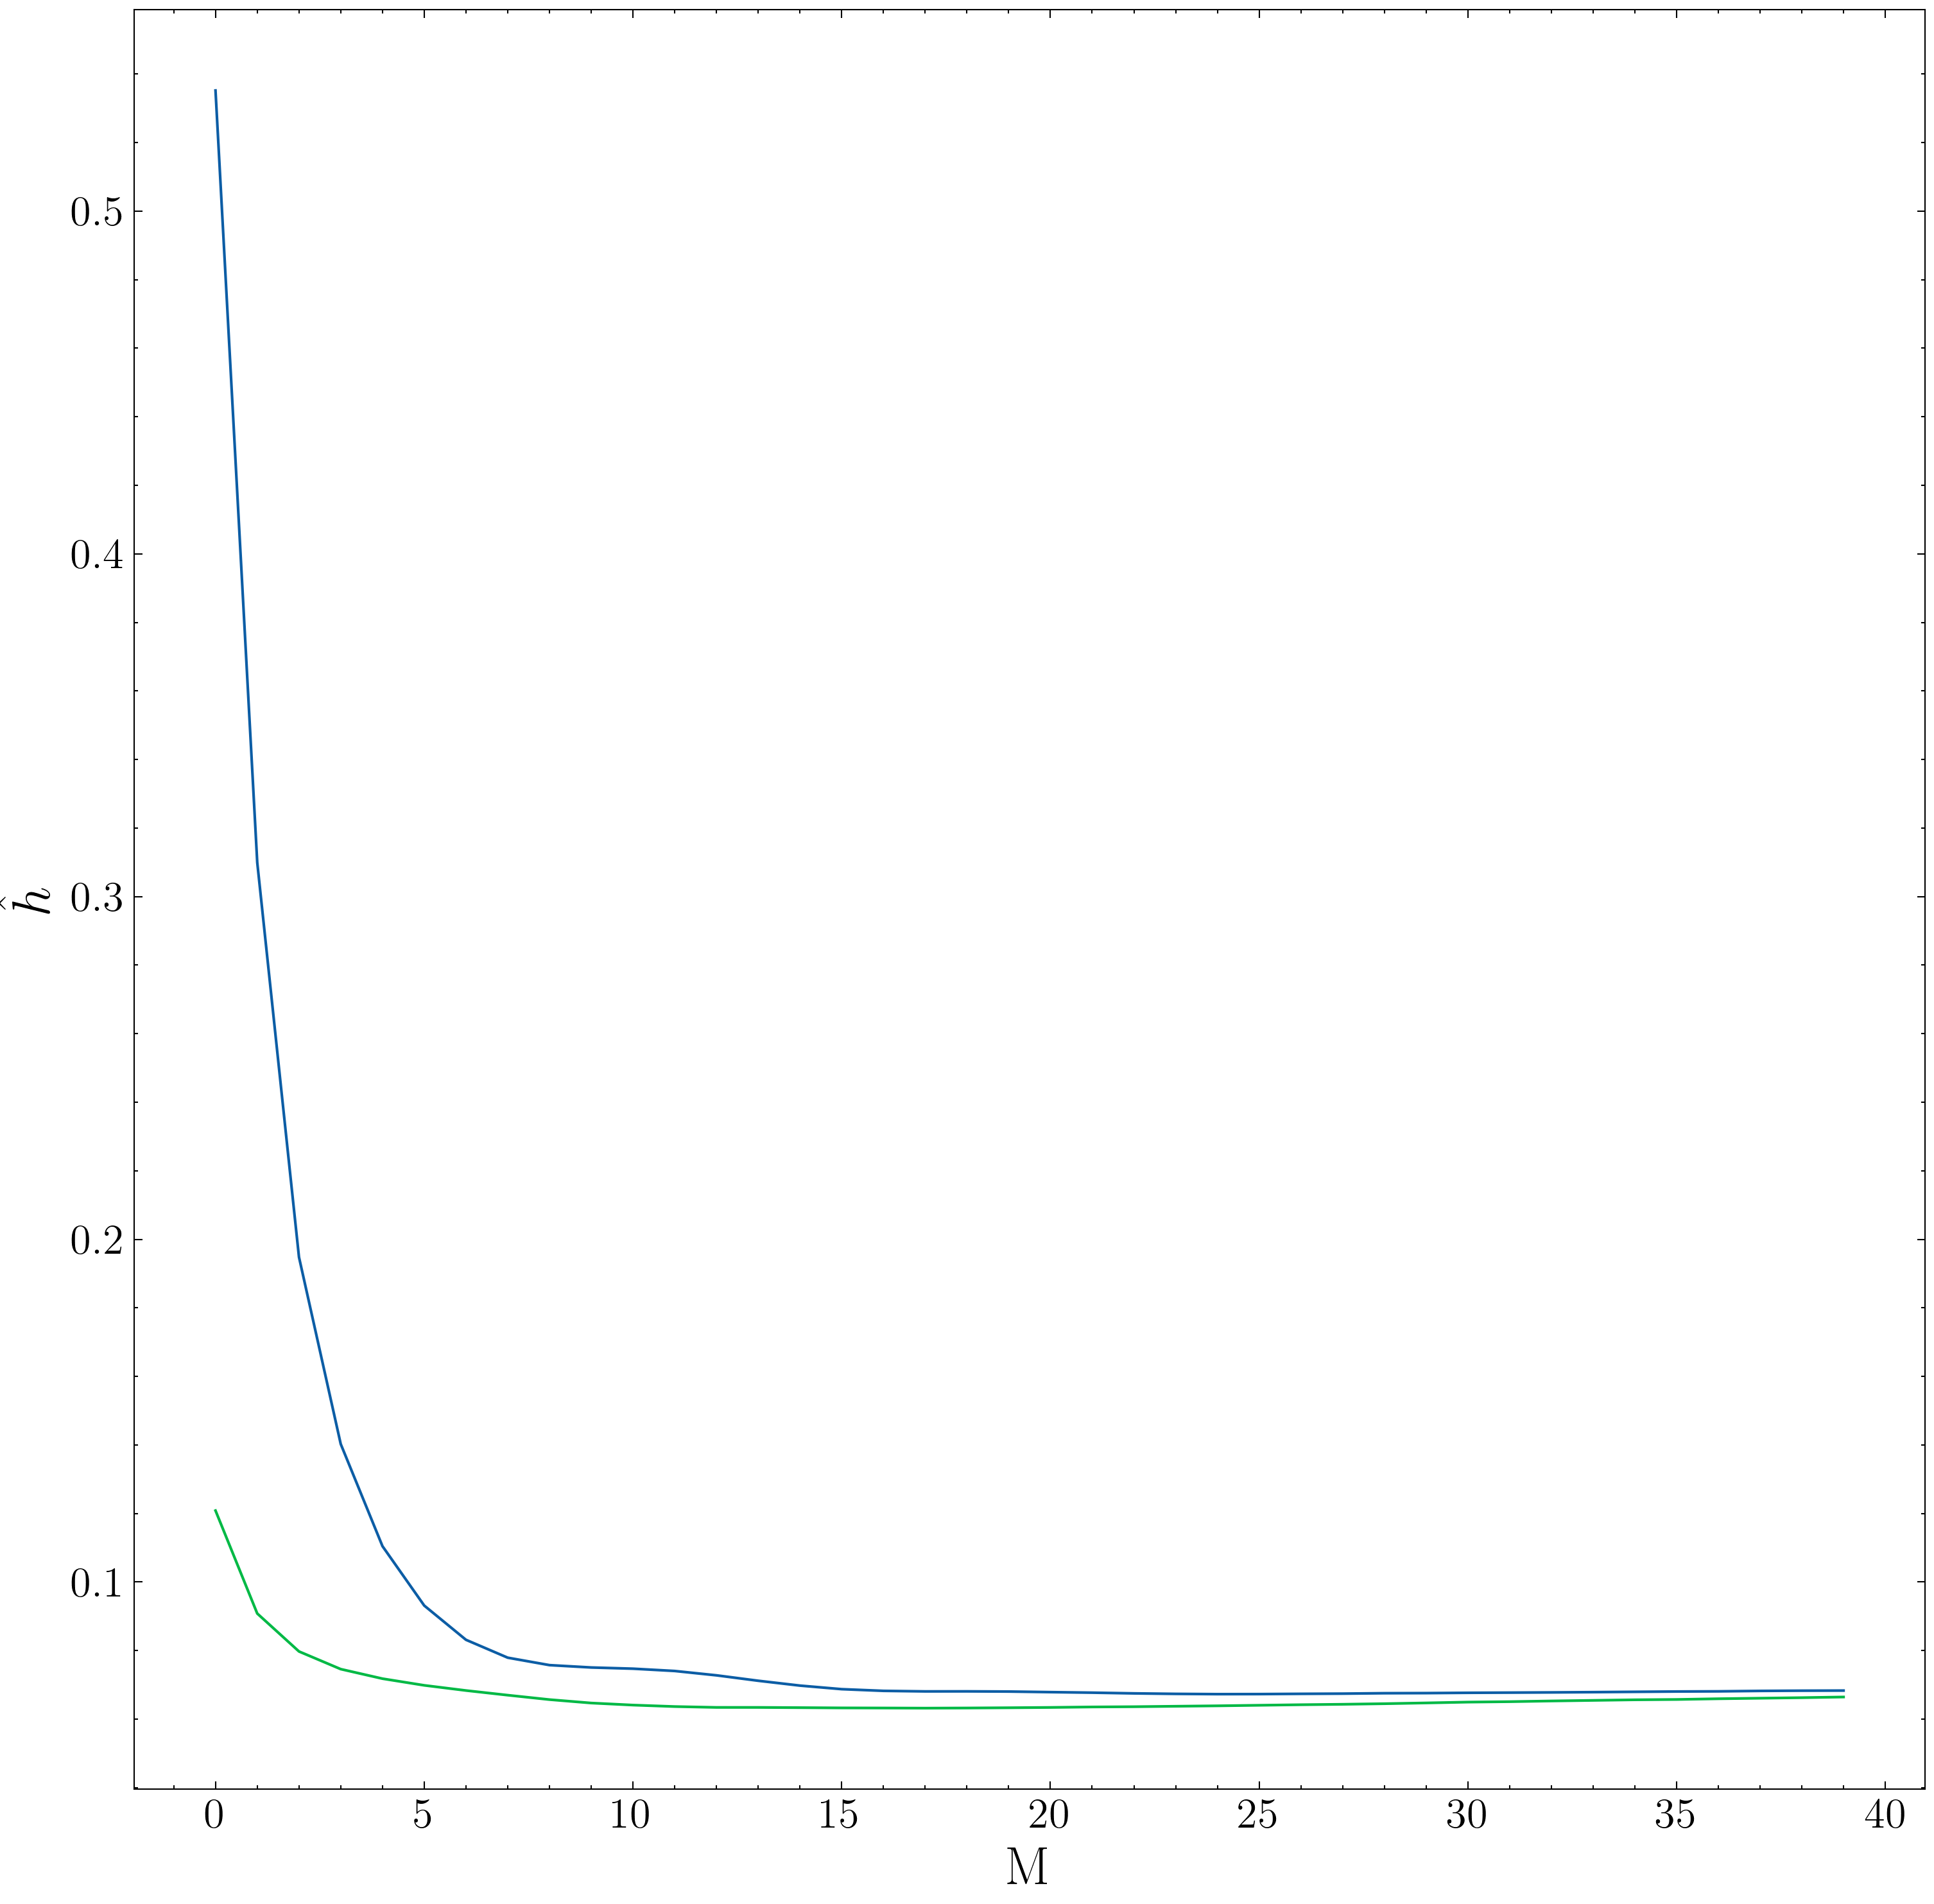
\includegraphics[width=\columnwidth]{images/filter_order.png}
%	\end{center}
%	\caption{\textcolor{red}{TK: filter order. From filter\_order\_experiments.mat. Maybe we should update this for an MSE after Viterbi?}}
%	\label{fig:filterorder}
%\end{figure}













%\begin{figure}
%	\begin{center}
%		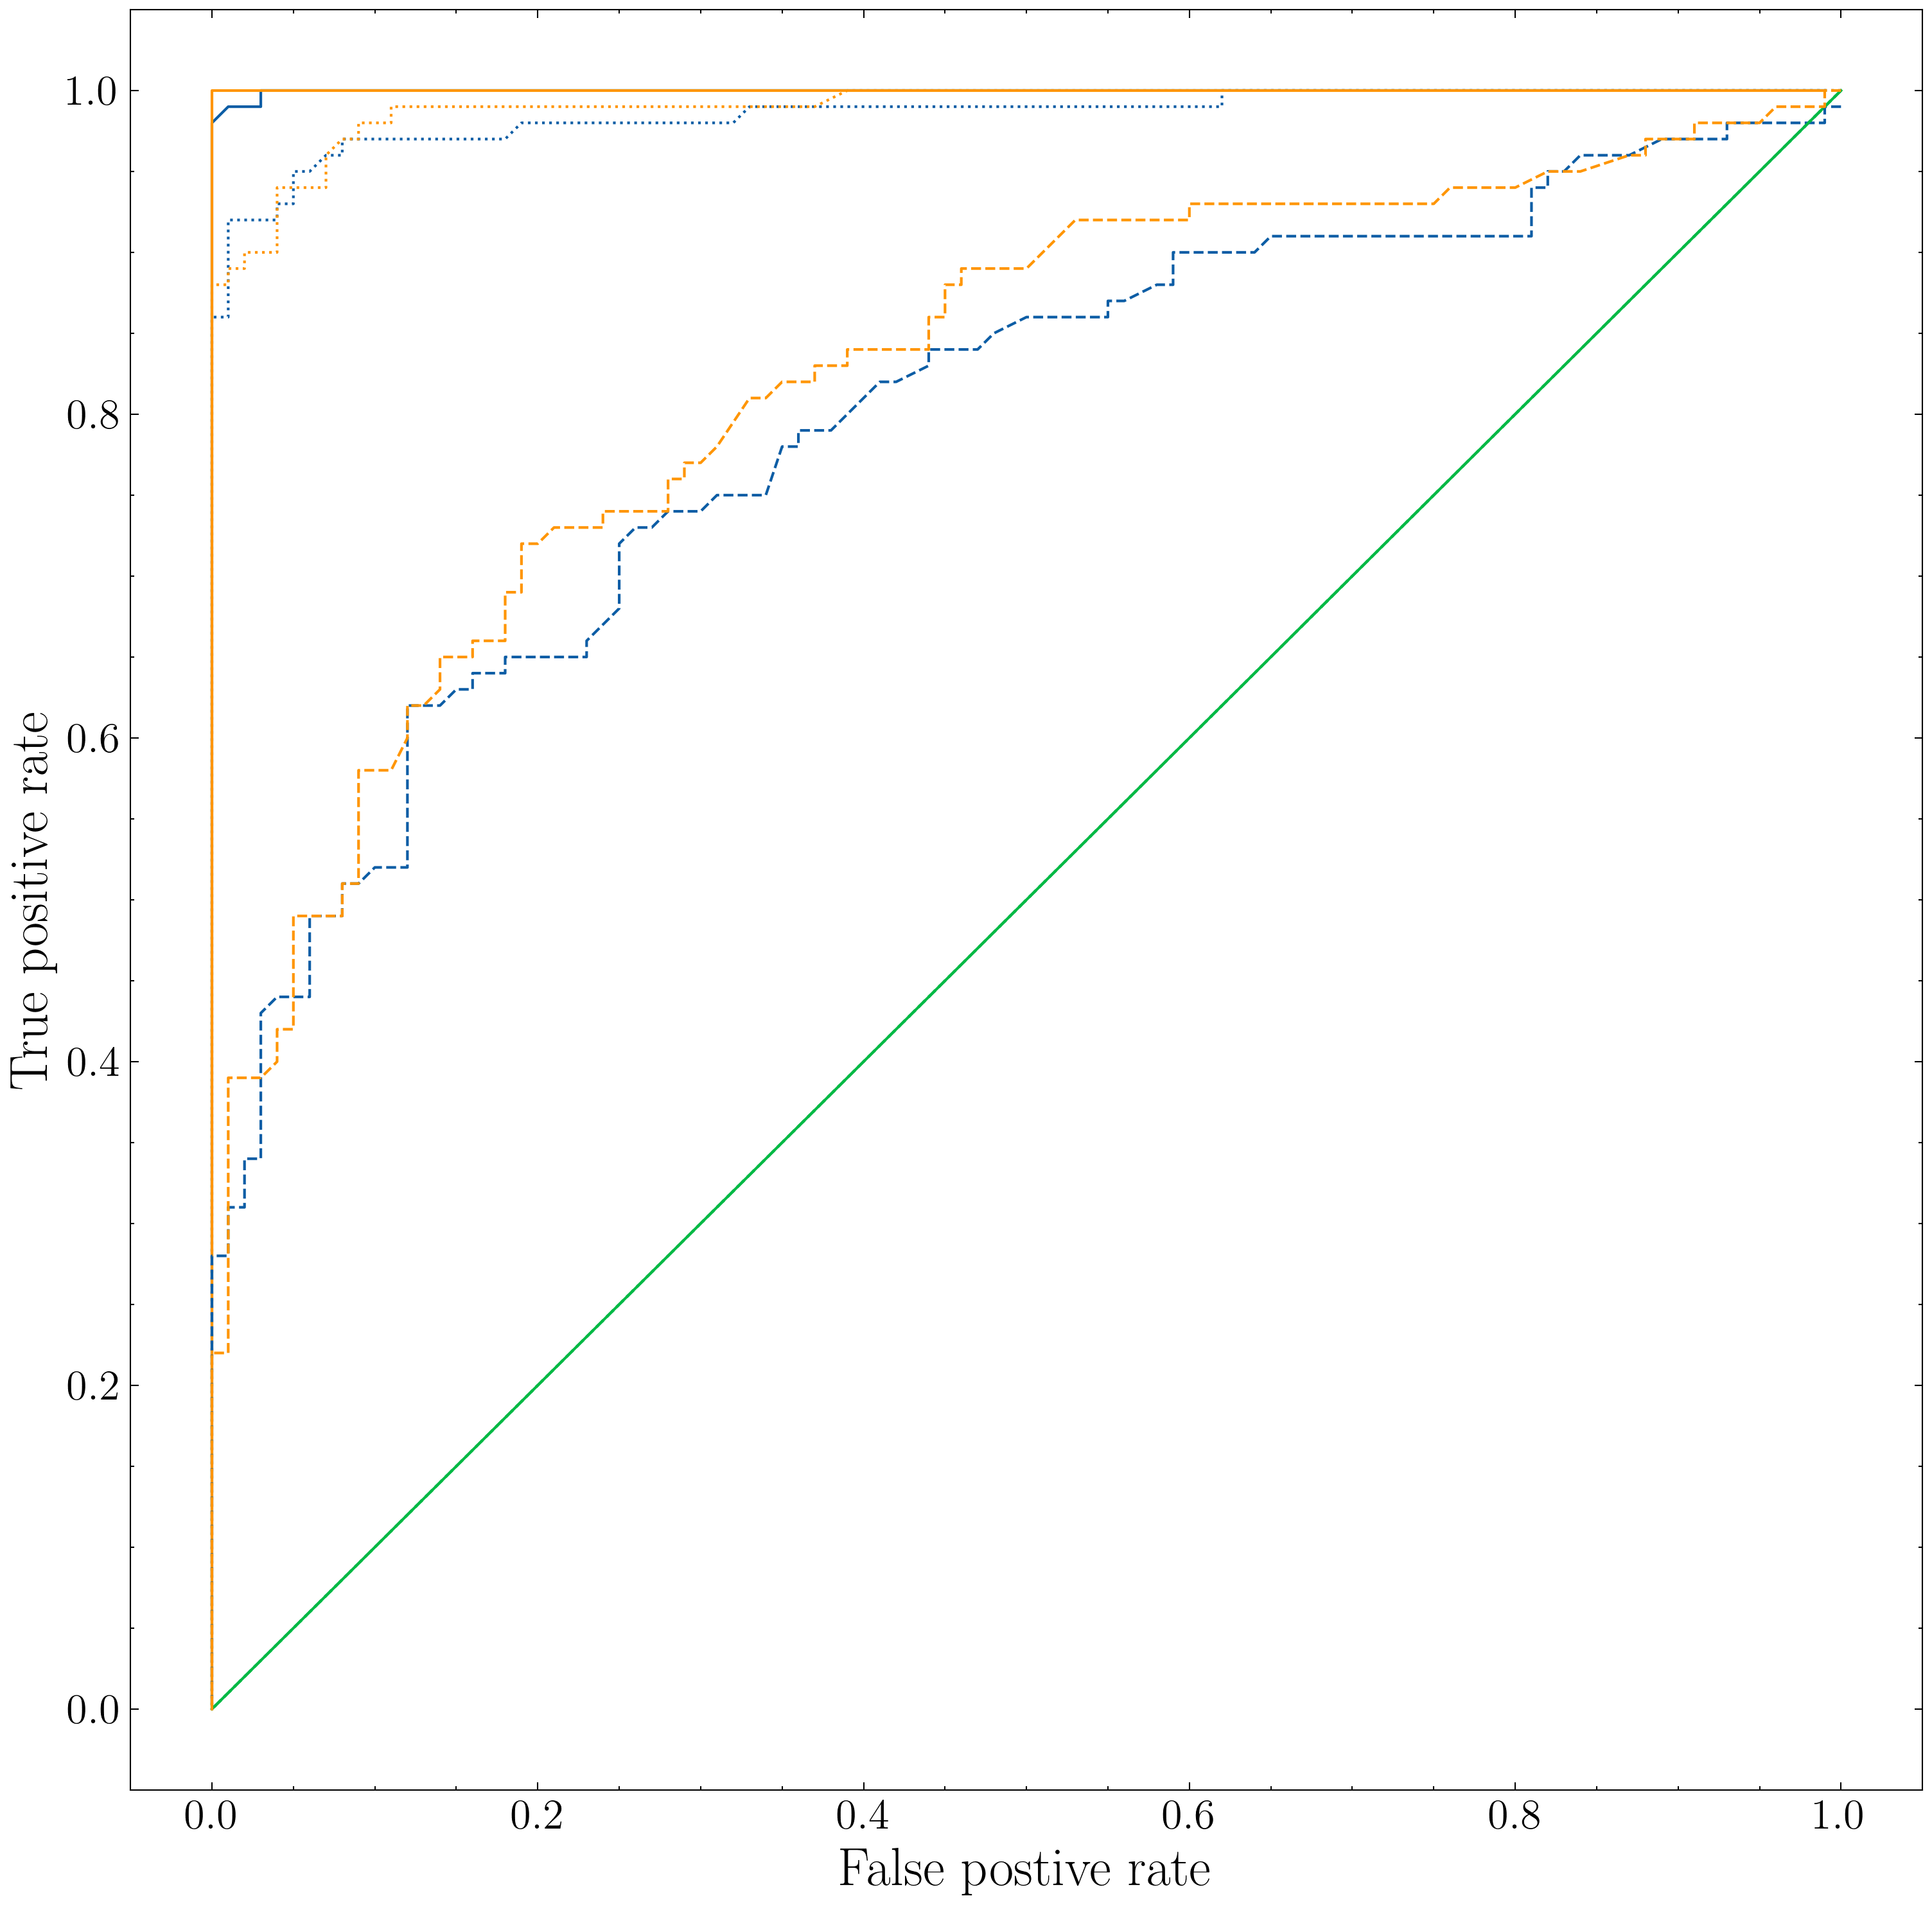
\includegraphics[width=\columnwidth]{images/roc_final_stacked.png}
%	\end{center}
%	\caption{ROC curve for 3 different systems $\{ \gamma = 0.001, \Delta f = 0.0\}$, $\{ \gamma = 0.01, \Delta f = 0.0\}$ , $\{ \gamma = 0.01, \Delta f = 0.5\}$ (dotted, dashed, solid respectively). The green lines denote the Viterbi search run without any ANC filtering, the blue lines with ANC filtering with 1 reference channel and the orange line with 2 reference channels. ANC filtering using 2 reference channels consistently outperforms that using a single reference channel.}
%	\label{fig:roc3}
%\end{figure}



%As discussed the ARLS filter has 2 parameters that can be freely chosen, the forgetting factor $\lambda$ and the model order (i.e. the number of taps in the FIR filter), $M$. For this work we have set $\lambda$ to a fixed value of $\lambda = 0.9999$. 




%
%
%

%\textcolor{red}{Changrong:} If we simply add more reference signals without normalizing the amplitude, it will definitely result in better performance (this is like we increase $|H(w)|$). But if we normalize the amplitude $a_r$ by $a_r/L$ with $L$ the number of references, we will not see obvious improvement.
%
%It might be the overfitting problem Rob mentioned previously, where with the number of taps chosen sufficiently large, it might already be enough to capture the dynamics of the interference signal without adding new interferences.
%
%But if we have multiple independent interference sources, with each reference correlated to each interference, then I suppose we should add more references.
%
%



\section{Conclusions}
In this paper we demonstrate a new line subtraction method based on adaptive noise cancellation for use in continuous gravitational wave searches. We use an adaptive recursive least squares method in conjunction with an independent, known PEM reference signal to suppress the interference from a long-lived narrow spectral feature. We then search for the continuous wave signal using a HMM Viterbi algorithm. We test our method on synthetic data containing the 60 Hz spectral interference line due to the North American power grid. We show how the the ANC and Viterbi algorithm together are able to successfully track the spin-wandering continuous GW signal near the 60 Hz line. We test the method over multiple noise realisations and show \textcolor{red}{TK: to confirm}. The performance of the filter is generally improved with an increased number of reference signals and at an increased model order. 






%This is a conclusion 




%\appendix
%\subfile{anc-app}
%\label{app:failedMs}


\newpage 
\newpage 

\appendix


%\begin{figure}[h!]
%	\begin{center}
%		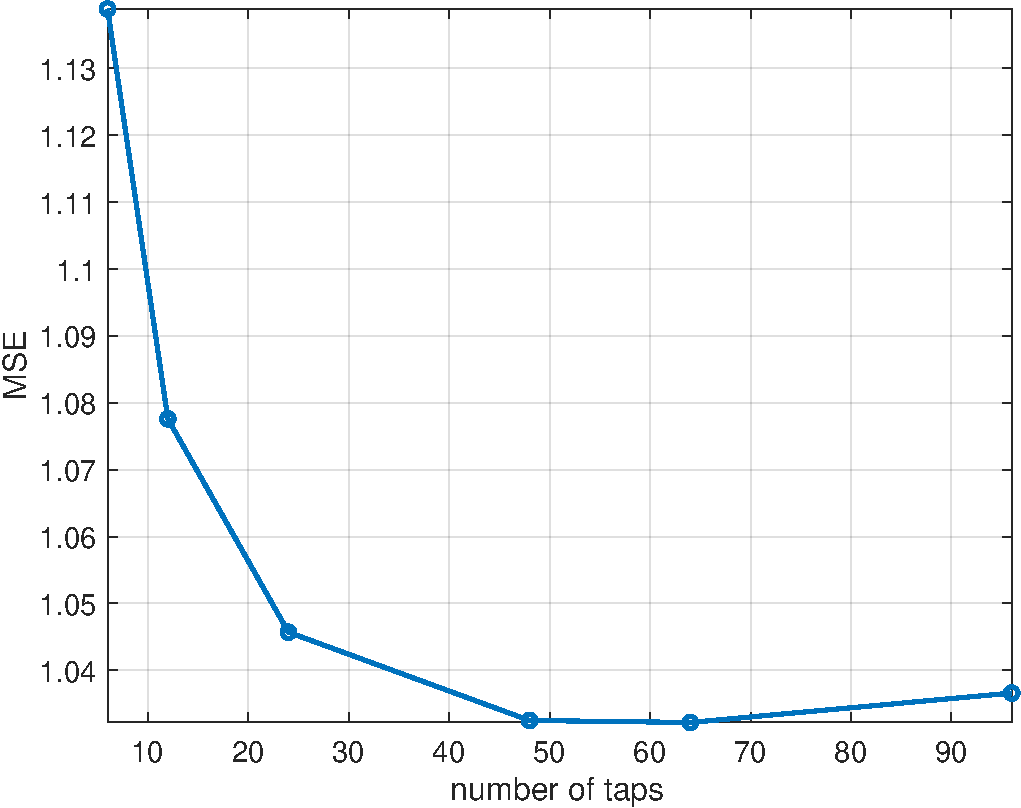
\includegraphics[width=0.49\textwidth]{result_images/mse_tap.pdf}
%	\end{center}
%	\caption{\label{mse vs tap}
%		Mean square error: MSE as a function of number of taps with $|H(w)|=3$ and $\rm{SNR}_{\rm in}=0.02$.}
%\end{figure}

















%
%\begin{figure*}
%	\begin{center}
%		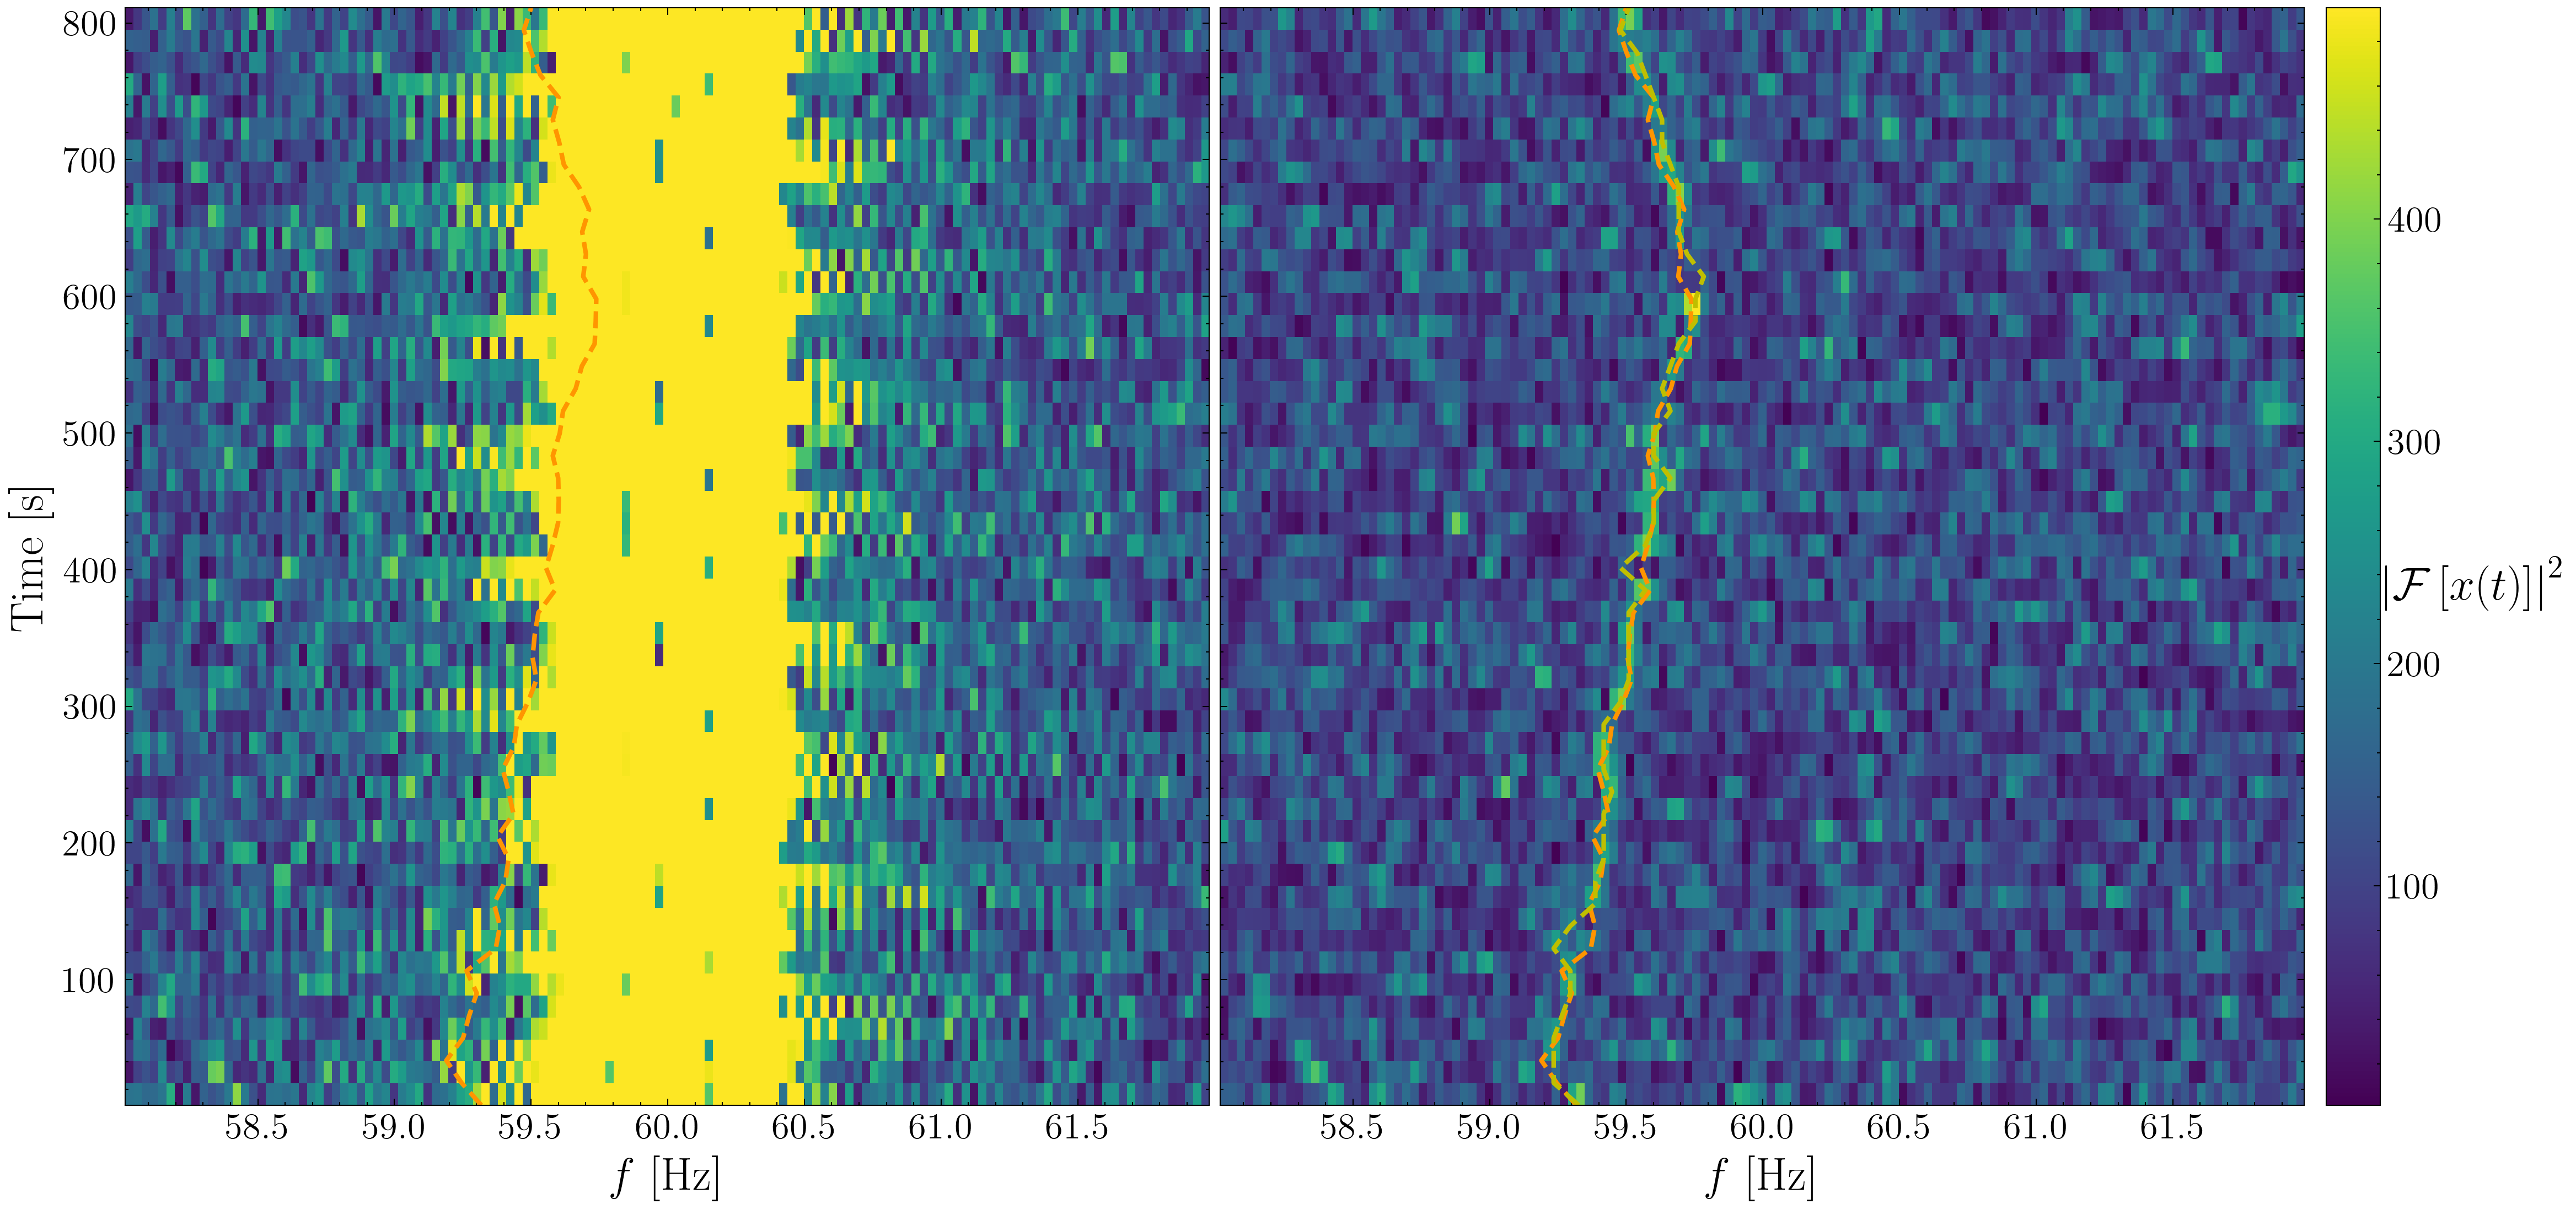
\includegraphics[width=\textwidth]{images/ANC_shared_y_example_1_high_contrast}
%	\end{center}
%	\caption{\label{frequency tracking before and after1high}
%		Tracking of the frequency evolution of a continuous GW with SNR$_{\rm in} = 0.025$, $H(\omega) =4$ and $\Delta f = 0.5$ using a HMM Viterbi algorithm both before (left hand panel) and after (right hand panel) the application of the ANC filter to remove the interference signal centred at 60Hz. The GW signal is indicated by diagonal dashed line. \textcolor{red}{TK: high contrast version also available. What are the settings?}}
%\end{figure*}
%
%
%
%\begin{figure*}
%	\begin{center}
%		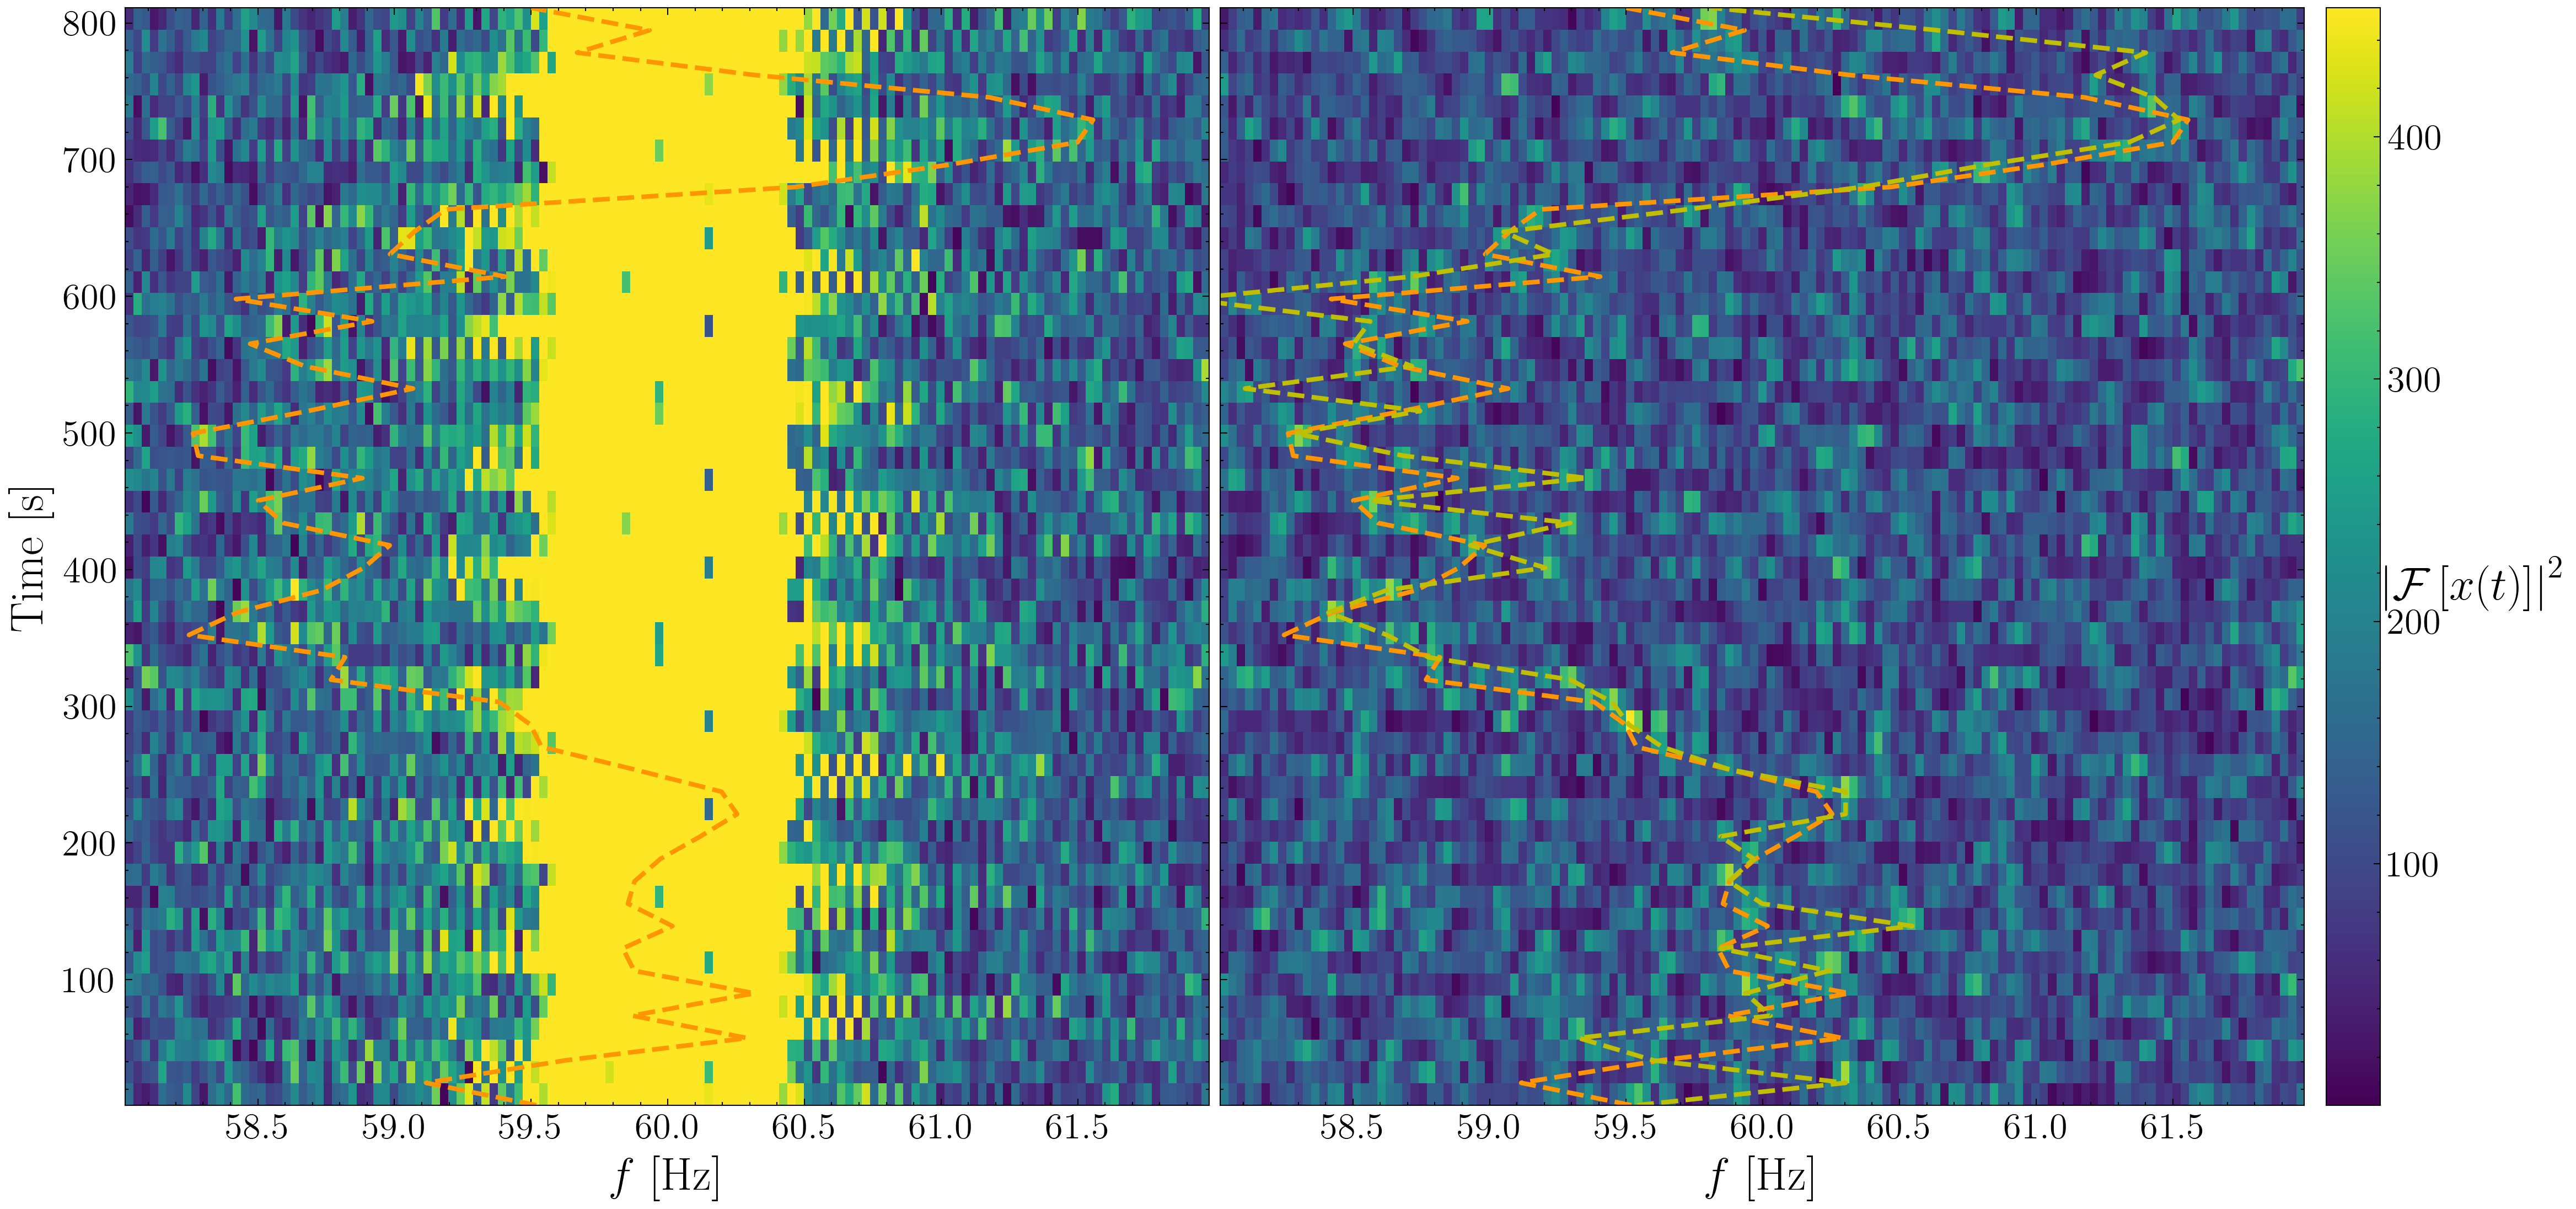
\includegraphics[width=\textwidth]{images/ANC_shared_y_example_2_high_contrast}
%	\end{center}
%	\caption{\label{frequency tracking before and after2high}
%		Tracking of the frequency evolution of a continuous GW with SNR$_{\rm in} = 0.025$, $H(\omega) =4$ and $\Delta f = 0.5$ using a HMM Viterbi algorithm both before (left hand panel) and after (right hand panel) the application of the ANC filter to remove the interference signal centred at 60Hz. The GW signal is indicated by diagonal dashed line. \textcolor{red}{TK: high contrast version also available. What are the settings?}}
%\end{figure*}
%
%
%




%
%
%
%
%\section{Old material}
%
%
%
%
%
%\begin{figure*}
%	\begin{center}
%		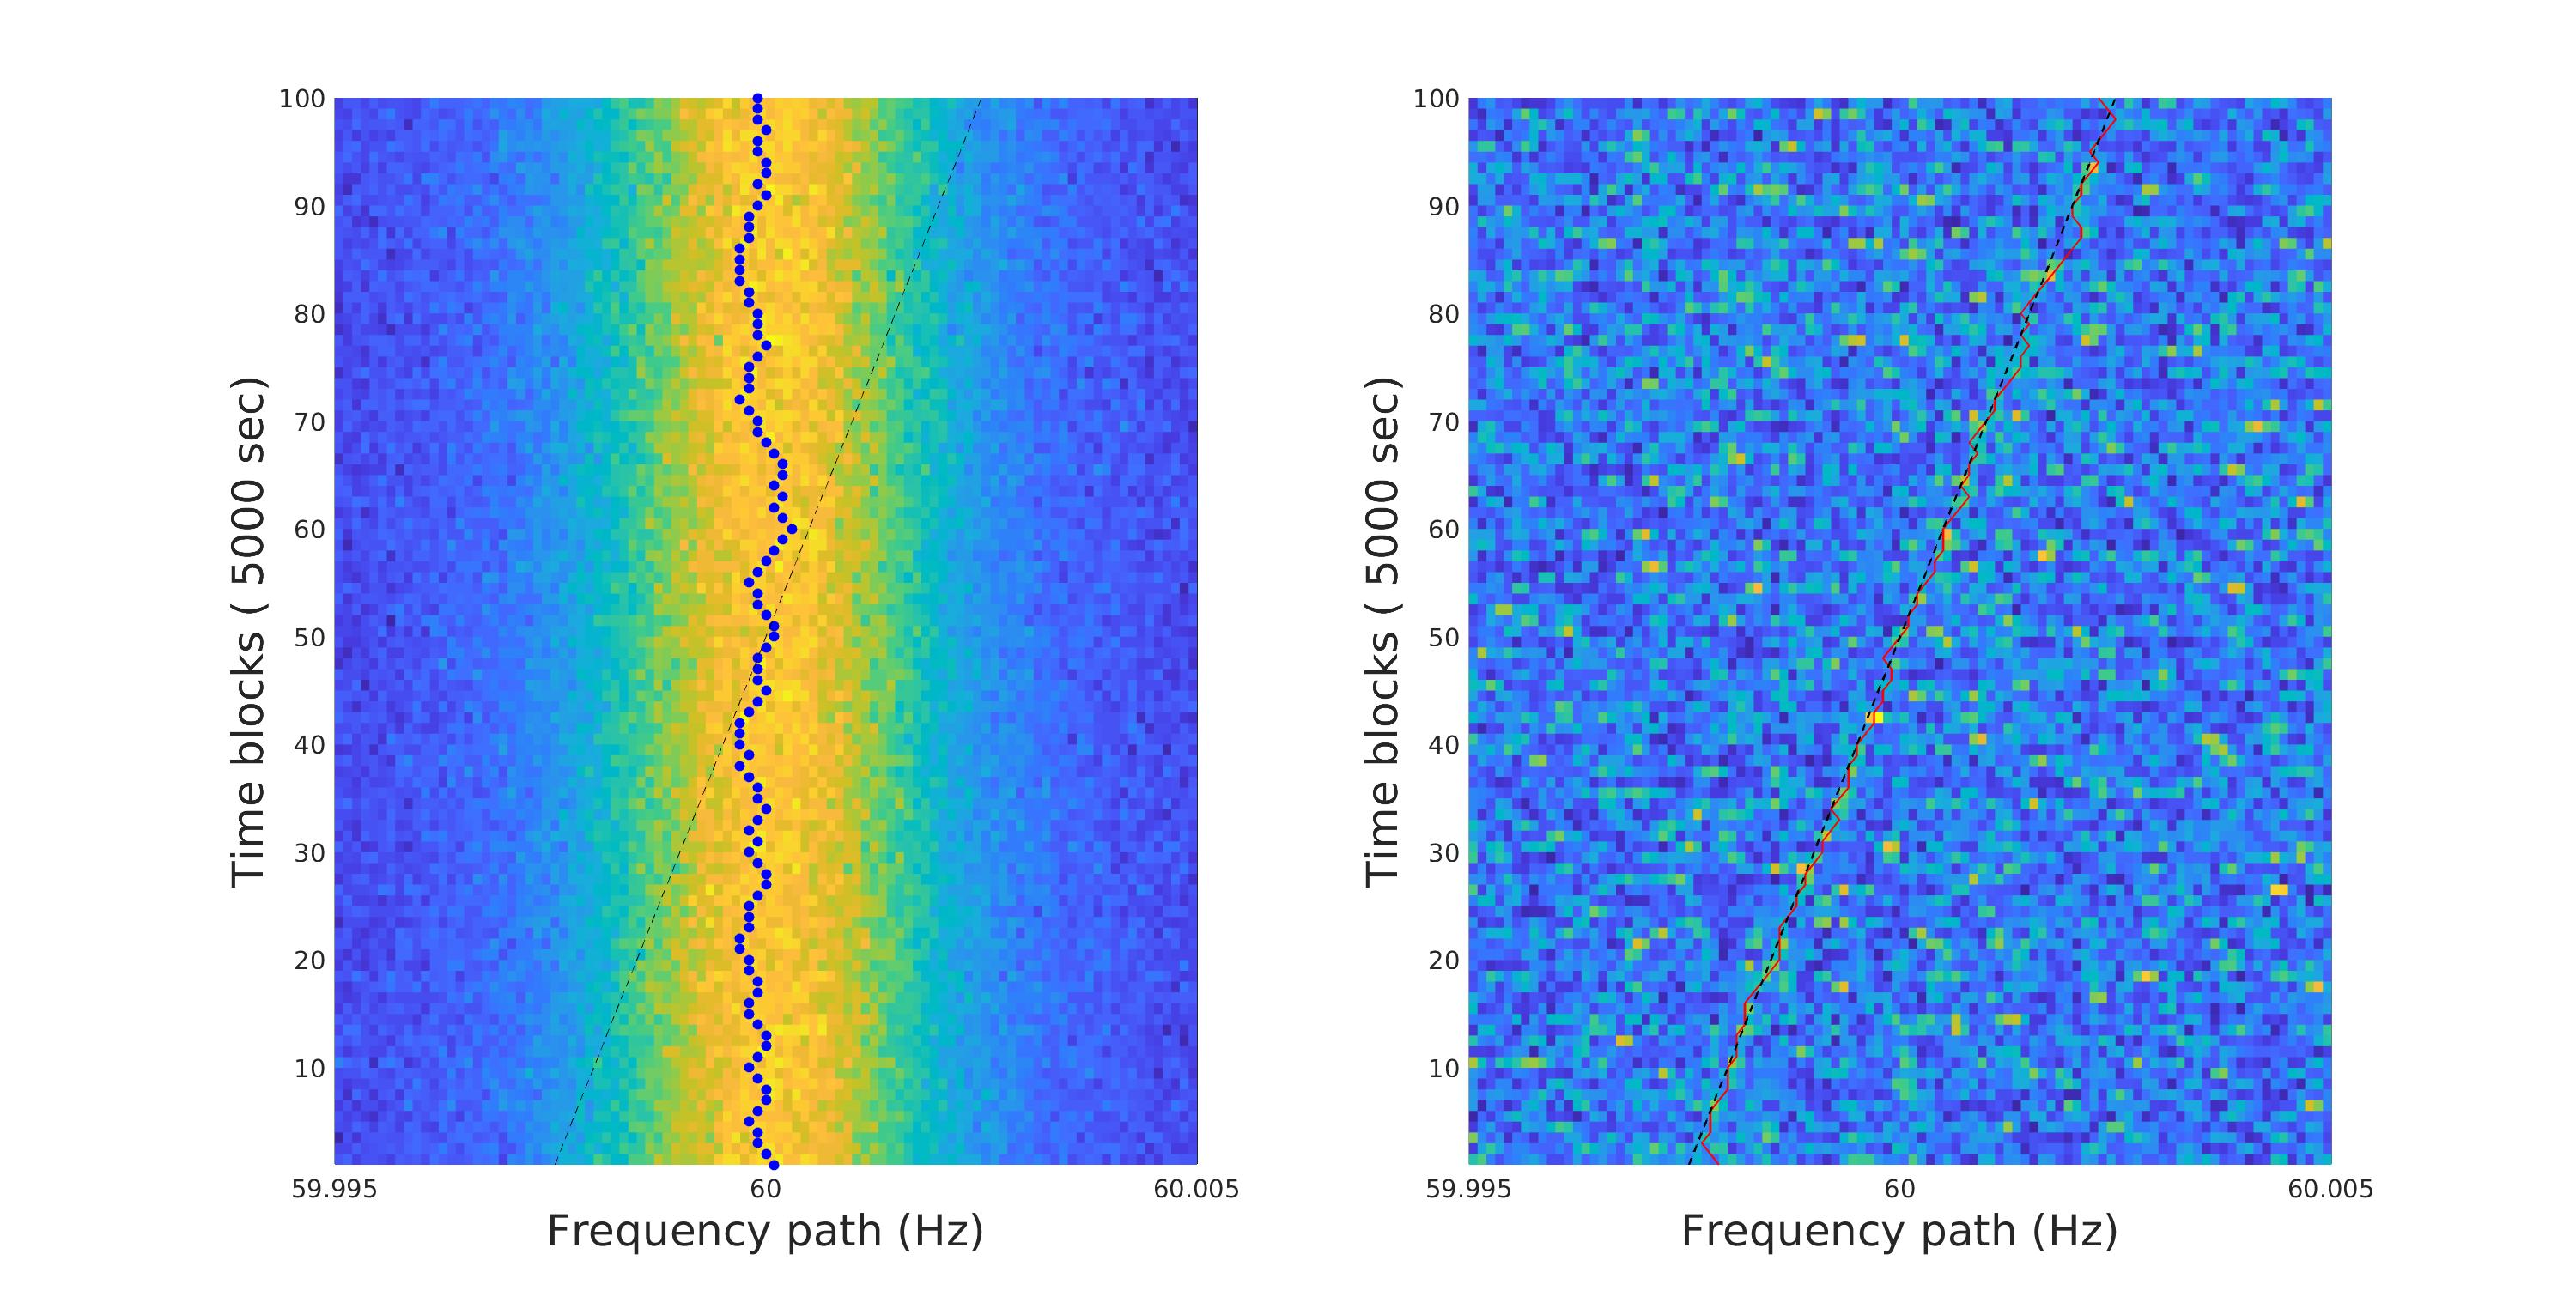
\includegraphics[width=\textwidth]{result_images/before_and_after.jpg}
%	\end{center}
%	\caption{\label{frequency tracking before and after}
%		Tracking of the frequency evolution of a continuous GW with SNR$_{\rm in} = 0.025$, $H(\omega) =4$ and $\Delta f = 0.5$ using a HMM Viterbi algorithm both before (left hand panel) and after (right hand panel) the application of the ANC filter to remove the interference signal centred at 60Hz. The GW signal is indicated by diagonal dashed line. \textcolor{red}{TK: What is the y axis? This should be two separate figures. Make red line clearer in RHS}}
%\end{figure*}
%
%
%
%
%\begin{figure}[h!]
%	\begin{center}
%		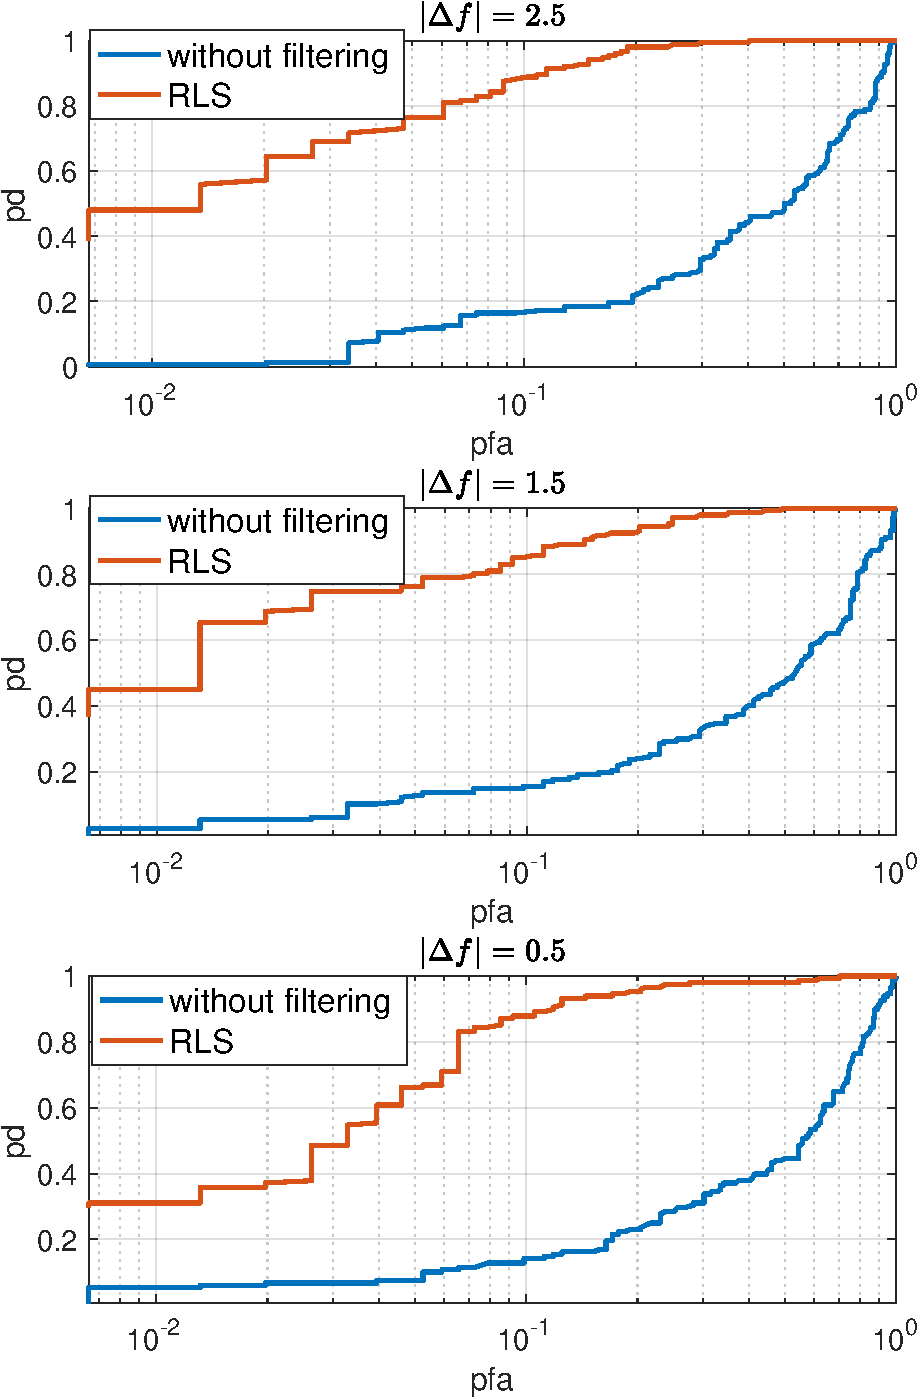
\includegraphics[width=0.49\textwidth]{result_images/frequency_difference_crop.pdf}
%	\end{center}
%	\caption{\label{fig:frequency difference}
%		ROCs under different $\Delta f$ with $|H(w)|=3$ and $\rm{SNR}_{\rm in}=0.025$}
%\end{figure}
%\begin{figure}[h!]
%	\begin{center}
%		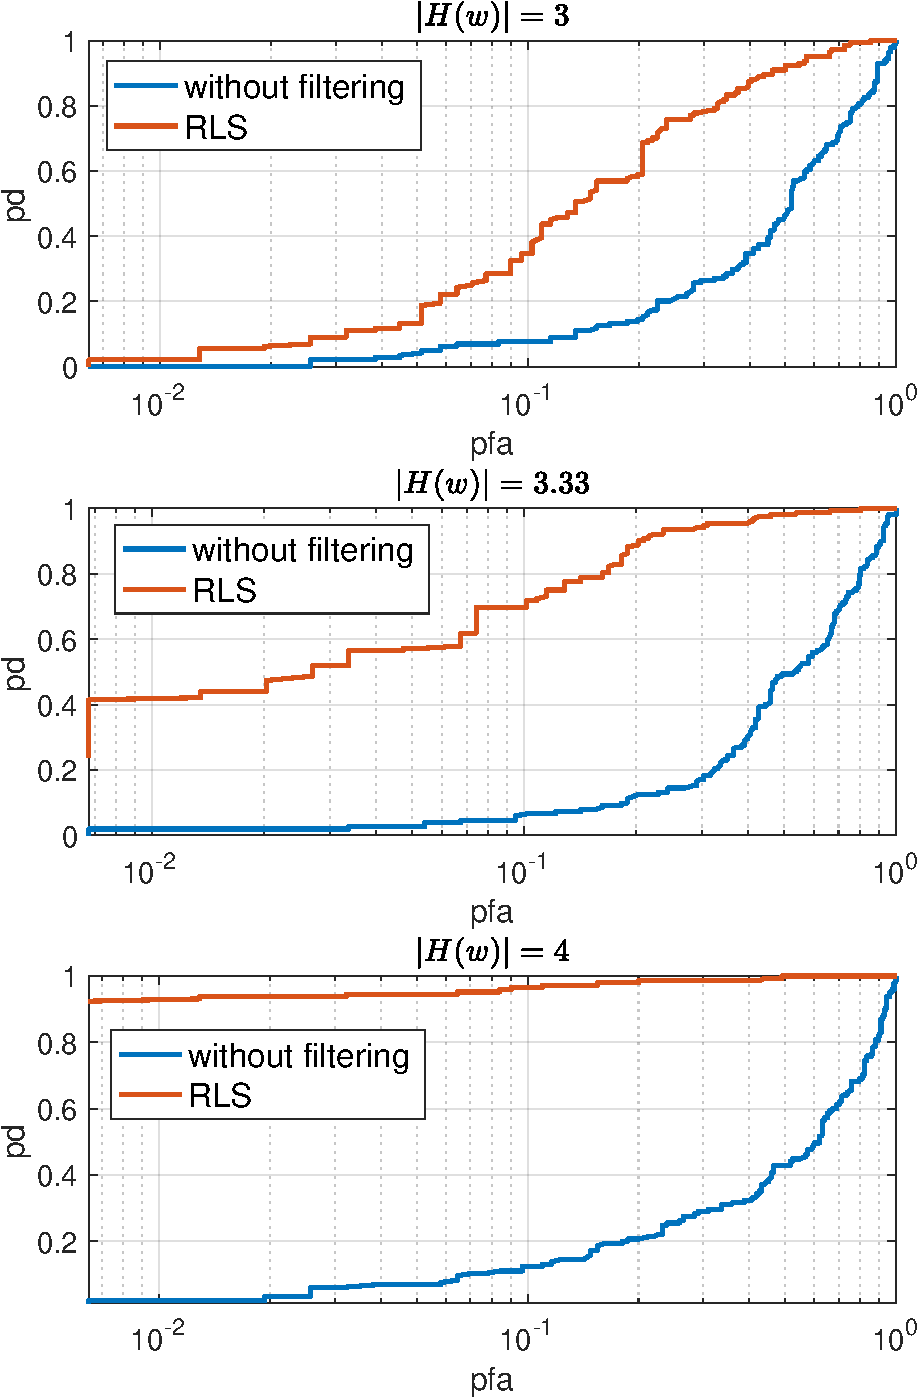
\includegraphics[width=0.49\textwidth]{result_images/homega_crop.pdf}
%	\end{center}
%	\caption{\label{fig:H(w)}
%		ROCs under different $|H(w)|$ with $\Delta f=0.5$ and $\rm{SNR}_{\rm in}=0.02$ \textcolor{red}{TK:change ordering of subplots so both delta f and H increase}}
%\end{figure}
%
%
%
%\begin{figure}
%	\begin{center}
%		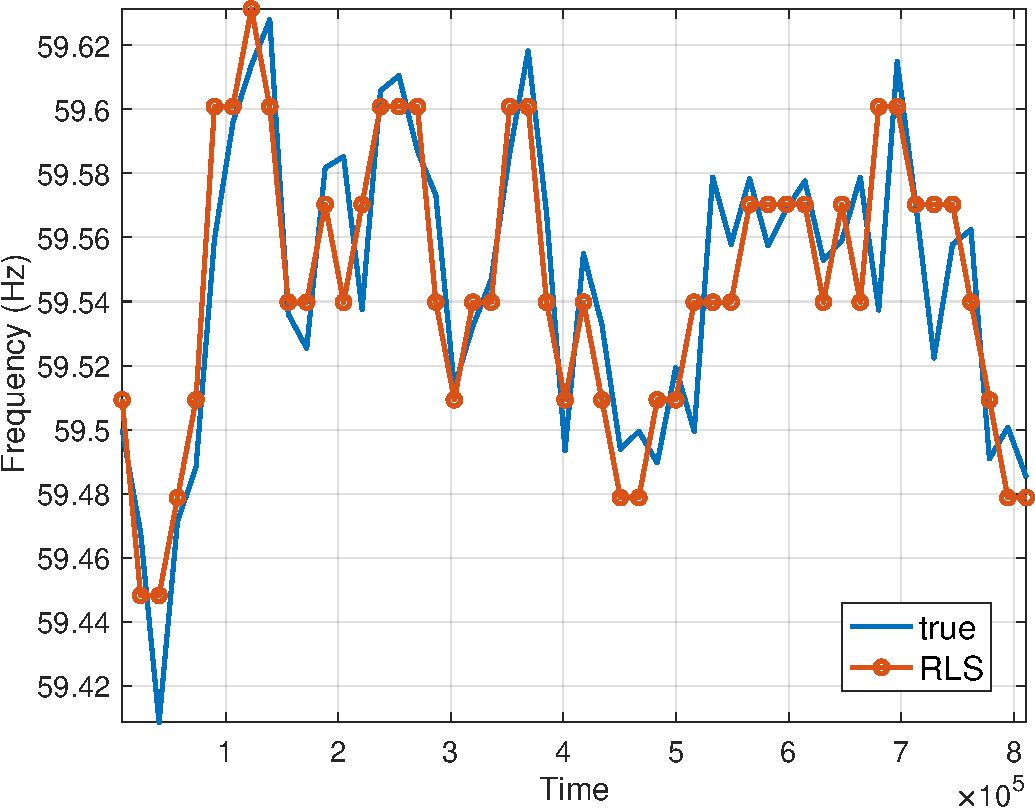
\includegraphics[width=0.49\textwidth]{result_images/frequency_tracking.pdf}
%	\end{center}
%	\caption{\label{frequency tracking}
%		Frequency tracking after RLS: $\rm{SNR}_{\rm in}=0.025$, $\Delta f = 0.5$, $|H(w)|=4$. \textcolor{red}{TK: Update this figure. Remove legend. Is this interference frequency or gw frequency?}}
%\end{figure}
%
%\begin{figure}
%	\begin{center}
%		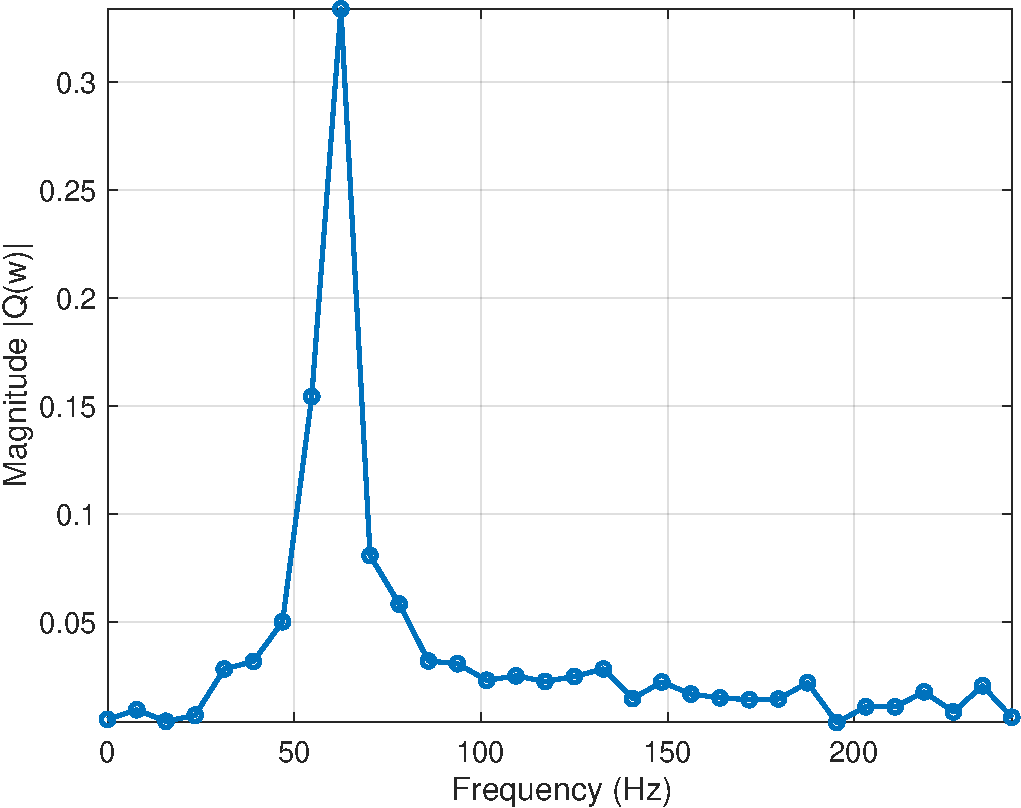
\includegraphics[width=0.49\textwidth]{result_images/taps2_frequency.pdf}
%	\end{center}
%	\caption{\label{taps_freq}
%		Frequency spectrum of the adaptive filter after converging. \textcolor{red}{TK: Update caption TBD}}
%\end{figure}
%
%
%\begin{figure}
%	\begin{center}
%		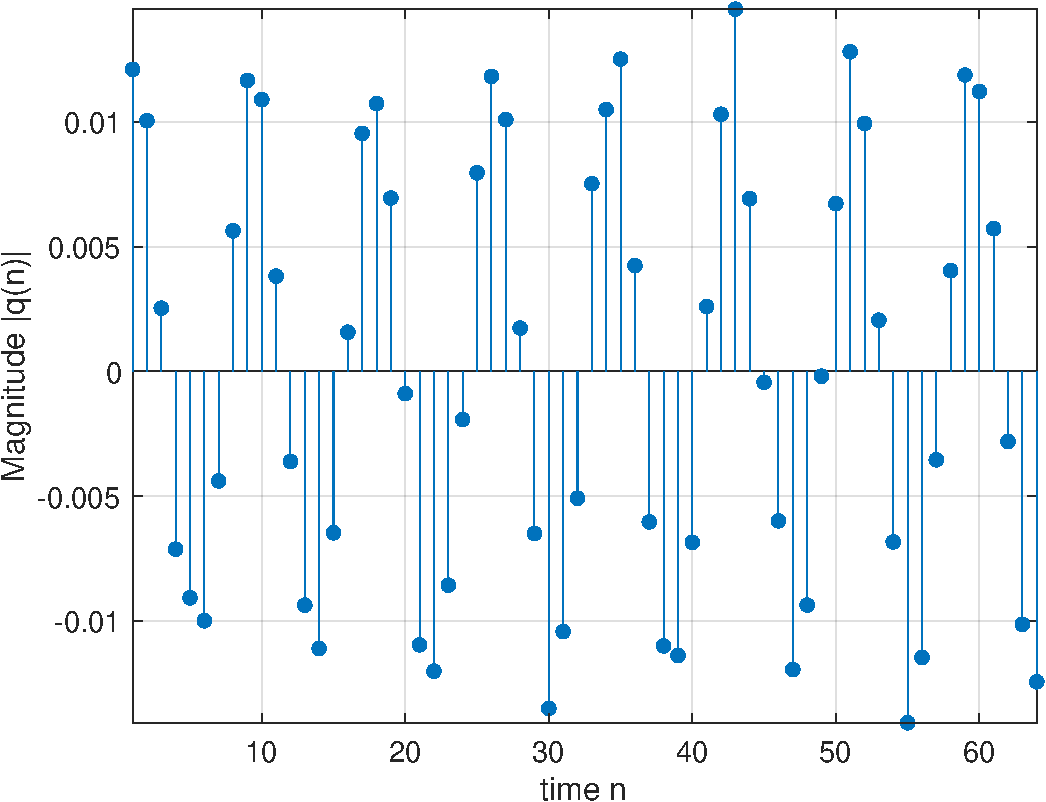
\includegraphics[width=0.49\textwidth]{result_images/taps2_time.pdf}
%	\end{center}
%	\caption{\label{taps}
%		Impulse response of the adaptive filter after converging. \textcolor{red}{TK: Clean up figure e.g. axis labels What is the x axis?}}
%\end{figure}




%\bibliographystyle{myunsrt}
\bibliographystyle{apsrev4-1} % Tell bibtex which bibliography style to use

\bibliography{bibLinesPaper}
%%%%%%%%%%%%%%%%%%%%%%%%%%%%%%%%%%%%%%%%%%%%%%%%%%


\begin{acknowledgements}
%GWOSC
This research has made use of data, software and/or web tools obtained from the Gravitational Wave Open Science Center (https://www.gw-openscience.org), a service of LIGO Laboratory, the LIGO Scientific Collaboration and the Virgo Collaboration. LIGO is funded by the U.S. National Science Foundation. Virgo is funded by the French Centre National de Recherche Scientifique (CNRS), the Italian Istituto Nazionale della Fisica Nucleare (INFN) and the Dutch Nikhef, with contributions by Polish and Hungarian institutes.
\end{acknowledgements}


\end{document}

